%Phần thiết đặt trang
\documentclass[12pt,a4paper]{article}
\usepackage{mathastext}
\usepackage[utf8]{vietnam}
\usepackage{amsfonts}
\usepackage{amsmath}
\usepackage{amssymb}
\usepackage{graphicx}
\usepackage[left=2cm,right=2cm,top=2cm,bottom=2cm]{geometry}
\setlength{\parindent}{0pt}
\usepackage{parskip}
\setlength{\parskip}{0.5em}

%Điều chỉnh nội dung bảng danh sách hình vẽ
\usepackage[titles]{tocloft}
\newlength{\mylen}
\renewcommand{\cftfigpresnum}{\figurename\enspace}
\renewcommand{\cftfigaftersnum}{:}
\settowidth{\mylen}{\cftfigpresnum\cftfigaftersnum}
\addtolength{\cftfignumwidth}{\mylen}

%Màu sắc cho bảng
\usepackage[table,xcdraw]{xcolor}

%Chuyển hình EPS sang dạng PDF tránh gây lỗi font
\usepackage{epstopdf}

%Cải thiện sắp xếp vị trí hình ảnh, dùng kèm với [H] trong phần option ảnh
\usepackage{float}

%Dùng dấu chấm thay dấu hai chấm trong caption ảnh
\usepackage[labelsep=period]{caption}

%Phần thiết kế khung code nhập liệu
\usepackage{listings}
\usepackage{color}

\definecolor{dkgreen}{rgb}{0,0.6,0}
\definecolor{gray}{rgb}{0.5,0.5,0.5}
\definecolor{mauve}{rgb}{0.58,0,0.82}

\lstset{frame=tb,
  language=Matlab,
  aboveskip=3mm,
  belowskip=3mm,
  showstringspaces=false,
  columns=flexible,
  basicstyle={\small\ttfamily},
  numbers=left,
  numberstyle=\small\color{gray},
  keywordstyle=\color{blue},
  commentstyle=\color{dkgreen},
  stringstyle=\color{mauve},
  breaklines=true,
  breakatwhitespace=true,
  tabsize=3
}

%Phần chọn font chèn câu lệnh giữa đoạn
\newenvironment{code}{\ttfamily}{\par}
\DeclareTextFontCommand{\chuyencode}{\code}

%Thêm chấm vào tiêu đề các phần
\usepackage{titlesec}
\titlelabel{\thetitle.\quad}

%Thêm định dạng cho các nút và menu lệnh.
\usepackage{menukeys}

%Đánh số cho các ví dụ và bài tập
\usepackage[thref,thmmarks,standard,amsmath,hyperref]{ntheorem}
\theoremheaderfont{\bfseries}
\theorembodyfont{\normalfont}
\theoremseparator{:}
\renewtheorem{example}{Ví dụ}

%Nội dung chính
\begin{document}
%Chỉnh loại tiêu đề chương thành I, II
\renewcommand\thesection{\Roman{section}}
\renewcommand\thesubsection{\arabic{subsection}}
\renewcommand\thesubsubsection{\alph{subsubsection}}

%Mục lục
\tableofcontents

%Chương 1:
\section{Cơ bản về MATLAB}
\subsection{Không gian làm việc}
\subsubsection{Giao diện chính}
Có 3 cách khởi động chương trình Matlab từ máy tính chạy Windows:\\
- Khởi động từ biểu tượng ngoài màn hình.\\
- Mở trực tiếp tập tin có đuôi mở rộng là .m, ví dụ: Bai1.m hoặc Hamso.m\\
- Vào biểu tượng Start $>$ All Program $>$ MATLAB $>$ Matlab 2014b.\\
\begin{center}
    \begin{figure}[htp]
    \begin{center}
     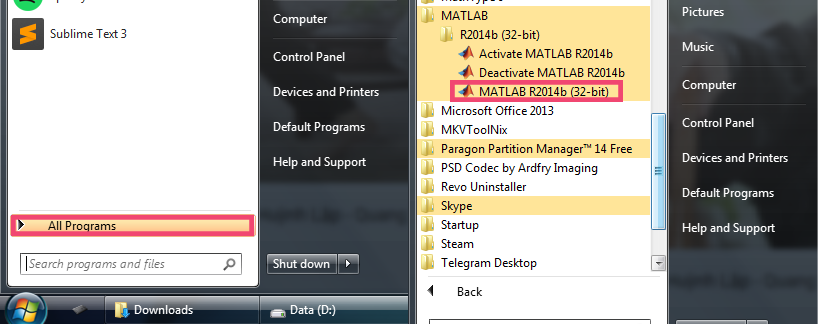
\includegraphics[scale=.7]{hinhtieuluan/pic1.png}
    \end{center}
    \caption{Thao tác mở chương trình từ Start Menu.}
    \label{refhinh1}
    \end{figure}
\end{center}
Giao diện chính của chương trình sau khi khởi động sẽ tương tự như hình bên dưới. Có 3 khu vực làm việc chính. Khung lớn nhất được bao viền màu xanh dương là Command Window. Khung Current Folder nằm ở phần trên, bên trái của Command Window. Phía dưới khung Current Folder là Khung Workspace.\\

\begin{center}
	\begin{figure}[htp]
	\begin{center}
		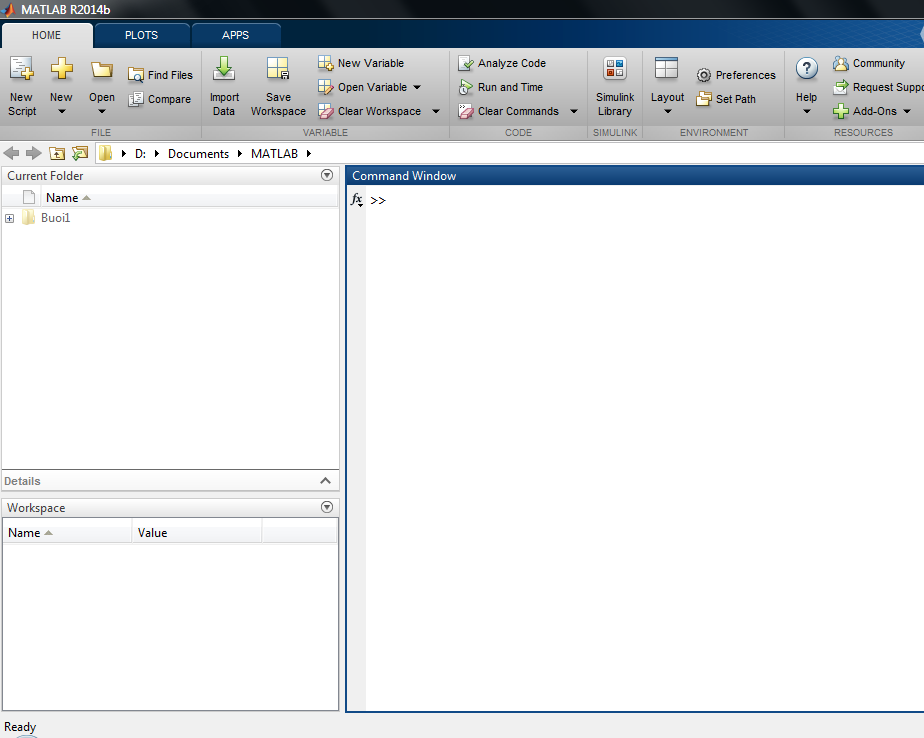
\includegraphics[scale=.6]{hinhtieuluan/pic2}
	\end{center}
		\caption{Giao diện chính của chương trình}
		\label{refhinh2}
	\end{figure}
\end{center}
Trong đó:\\
\begin{itemize}
	\item \textbf{Command Window:} Khu vực người dùng nhập các câu lệnh điều khiển và tính toán. Mỗi câu lệnh sẽ được thực hiện khi người dùng nhấn Enter.
	\item \textbf{Current Folder:} Khu vực truy cập các tập tin m-file, m-hàm... được lưu trữ trên ổ đĩa máy tính.
	\item \textbf{Workspace:} Liệt kê các biến và dữ liệu đang được xử lý tạm thời. Ngoài ra người dùng có thể thao tác thêm bớt chỉnh sửa các giá trị của biến và tham số trực tiếp trên Workspace mà không cần dùng đến câu lệnh.
\end{itemize}
Ngoài ba khu vực chính trên, kể từ phiên bản MATLAB 2012a, thanh công cụ phía trên cùng truyền thống đã được thay thế bằng các thẻ lệnh Ribbon với biểu tượng cụ thể và rõ ràng hơn.\\
\begin{center}
	\begin{figure}[htp]
		\begin{center}
		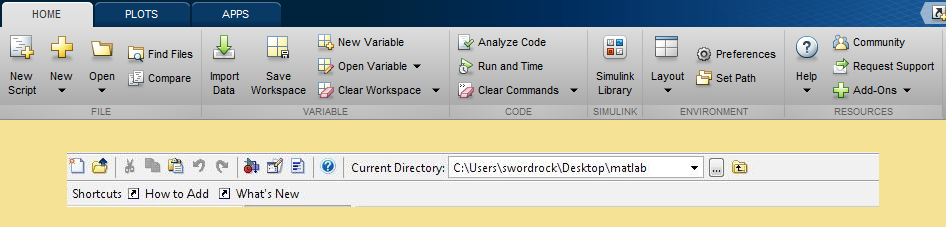
\includegraphics[scale=.5]{hinhtieuluan/pic3}
		\end{center}
		\caption{Thẻ Home (hình trên) và thanh công cụ truyền thống (hình dưới)}
		\label{refhinh3}
	\end{figure}
\end{center}
\subsubsection{Các thao tác cơ bản}
MATLAB thực hiện các phép cộng, trừ, nhân, chia như một chiếc máy tính bình thường. Xét các ví dụ đơn giản sau:\\
\begin{example}
	Tính 3 + 2 + 6; 4 x 6 x 25 + 32 - 9 : 3.
	\begin{lstlisting}
	>> 3 + 2 + 6 =
	ans =
				12
	>> 4 * 6 * 25 + 32 - 9 / 3 =
	ans =
				629
	\end{lstlisting}
\end{example}

\textbf{Lưu ý:} MATLAB không quan tâm đến khoảng trắng giữa các dấu và luôn ưu tiên phép nhân rồi mới đến phép cộng. Kí hiệu \chuyencode{ans} là viết tắt của từ "answer" có nghĩa là kết quả của phép tính.\\
\begin{example}
	Tính $sin{\dfrac{\pi}{2}}+cos{\dfrac{\pi}{2}}$\\
	\begin{lstlisting}
	>> sin(\pi/2)+cos(\pi/2)=
	ans =
				1
	\end{lstlisting}
\end{example}
\subsection{Biến, hằng số, hàm cơ bản}
Trong MATLAB, ta có thể gián giá trị cho biến với tên gọi bất kỳ, điều này giúp cho việc tính toán rõ ràng vả dễ dàng hơn. Đặt biệt với những bài tính toán với các biến số, ta dễ dàng thay đổi giá trị của biến số để có được các kết quả phù hợp với yêu cầu tính toán.\\
\textbf{Yêu cầu khi đặt tên biến:} Tên biến phải bắt đầu bằng chữ cái, các ký tự sau ký tự đầu tiên có thể là số, chữ hoặc ký tự "\_". Tên biến có độ dài tối đa là 31 ký tự, trong tên biến không được dùng dấu chấm câu. Ngoài ra, MATLAB phân biệt ký tự hoa sẽ khác với ký tự thường. Tức là biến "var1" sẽ khác với biến "Var1".\\
Một số biến đã được định nghĩa sẵn (một số còn được gọi là hằng số):
\begin{itemize}
	\item Ký tự i và j được dùng cho đơn vị phức.
	\item Biến eps dùng để chỉ số nhỏ nhất, số này khi cộng với 1 ta được số nhỏ nhất lớn hơn 1.
	\item Biến pi dùng để chỉ số pi ($\pi$), với giá trị là 3.1415926...
	\item Biến ans dùng để lưu kết quả vừa tính toán trước đó.
	\item Biến Inf và -Inf (lưu ý ký tự I đứng đầu được viết hoa) dùng để biểu diễn dương và âm vô cực.
	\item Ký tự NaN thể hiện cho "Not a Number", không phải là một số.
\end{itemize}
\textbf{Biến thông thường:} (hay còn được gọi là biến vô hướng) là biến được người dùng định nghĩa bằng cách gián một giá trị cụ thể nào đó trực tiếp thông qua câu lệnh trong Command Windows.
\begin{example}
\normalfont
Tạo biến tên a chứa giá trị là số 10. Ta sẽ nhập lệnh vào Command Windows như sau:
\begin{lstlisting}
	>> a = 10
	a =
    		10
\end{lstlisting}
Ngay lập tức biến tên a sẽ được liệt kê trong khu vực Workspace. Người dùng có thể truy cập hoặc điều chỉnh giá trị biến ngay trong cửa sổ Workspace.\\
\begin{center}
	\begin{figure}[htp]
		\begin{center}
		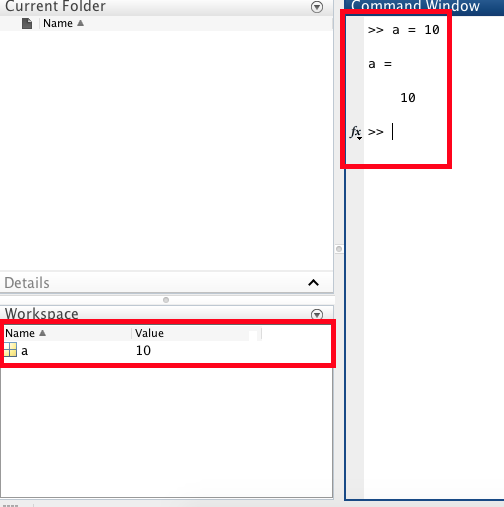
\includegraphics[scale=.5]{hinhtieuluan/pic4}
		\end{center}
		\caption{Tạo biến ở khu vực Command Window và quản lý biến tại khu vực Workspace.}
		\label{refhinh4}
	\end{figure}
\end{center}
\end{example}
\begin{example}
\normalfont Tạo biến c dựa vào biến a có sẵn biết rằng c được tính qua biểu thức $c=a^2+a^3$. Ta tiếp tục nhập lệnh sau vào khu vực Command Window từ ví dụ trước đó:
\begin{lstlisting}
	>> c = a^2 + a^3
	c =
        	1100
\end{lstlisting}
Qua ví dụ 2 ta có thể tạo biến dựa vào giá trị của một biến khác cho trước. Ngoài ra, ta có thể ẩn đi kết quả tính toán của câu lệnh bằng cách thêm dấu ";" vào cuối câu lệnh. Ví dụ sau sẽ giúp ta dễ hình dung:
\begin{lstlisting}
	>> b = 6 + c;
	>> b = 6 + c
	b =
        	1106
\end{lstlisting}
\end{example}


\subsection{Quản lý tập tin, M-file}
\subsubsection{Tạo thư mục lưu trữ}
Trong MATLAB, ta nên tập thói quen dùng các thư mục được sắp xếp gọn gàng để phân loại dữ liệu đang xử lý. Những thao tác cơ bản gồm:
\begin{itemize}
	\item Để tạo thư mục mới, chọn nút "Browse for folder" ở gần khu vực Current Folder. Sau đó ta tạo thư mục mới trong cửa sổ vừa hiện ra, đặt tên cho thư mục (lưu ý rằng tên thư mục không được phép chứa ký tự khoảng trắng).
	\item Chọn thư mục vừa tạo và nhấn nút "Open" để mở.
	\item Lúc này, thư mục hiện hành chính là thư mục bạn vừa mới tạo.
	\item Không chỉ cho phép người dùng tạo thư mục thông qua cửa sổ "Browse for folder", người dùng còn có thể xoá, sửa hay di chuyển thư mục trong cửa sổ đó.
\end{itemize}
\textbf{Nâng cao:} Với những người dùng thường xuyên lưu trữ chương trình hoặc các tập tin m-file ở các thư mục nằm nhiều nơi trên ổ đĩa, người dùng có thể thêm đường dẫn thư mục đó vào cửa sổ \textbf{Set Path (trong phần Enviroment)} để có thể chạy lệnh tính toán mà không cần quan tâm vị trí lưu trữ thư mục chứa các tập tin đó.
\subsubsection{Scripts (Đoạn mã lệnh)}
Scripts (còn được gọi là đoạn mã lệnh) là một tập tin chứa các câu lệnh chạy trong môi trường MATLAB. Các câu lệnh được lưu trữ trong tập tin này sẽ được thực thi theo trình tự.\\
Scripts được viết trong cửa sổ MATLAB Editor tích hợp sẵn trong MATLAB và được lưu trên ổ đĩa dưới dạng các tập tin có đuôi mở rộng là .m, dung lượng thường không quá 100MB. Ngoài ra, ta hoàn toàn có thể dùng một công cụ soạn thảo cơ bản như \textbf{Notepad} mặc định của Windows để tạo ra một tập tin đuôi .m nhưng yêu cầu các câu lệnh trong đó phải đúng và thực thi được trong môi trường MATLAB.\\
Các cách tạo một tập tin MATLAB (đuôi .m):
\begin{itemize}
	\item Từ Command Windows gõ câu lệnh với cú pháp \chuyencode{edit tenfile.m}, trong đó ta thay thế \chuyencode{tenfile.m} bằng tên tập tin muốn tạo. Sau đó chọn OK trong cửa sổ xác nhận tạo tập tin \chuyencode{tenfile.m}.
	\item Chọn vào biểu tượng \textbf{New Script} trong khu vực \textbf{File} hoặc chọn \menu{File > New > Script} đều được. Sau khi cửa sổ soạn thảo đã mở, ta chọn biểu tượng \textbf{Save} trong khu vực File và tiến hành đặt tên cho tập tin cùng với việc chọn khu vực lưu trữ.
\begin{center}
	\begin{figure}[htp]
		\begin{center}
		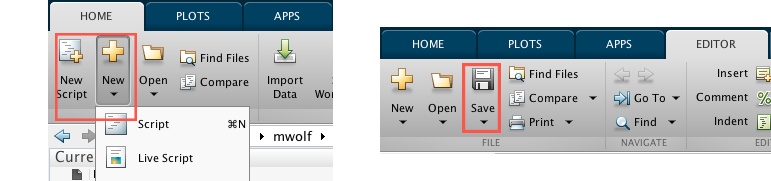
\includegraphics[scale=.5]{hinhtieuluan/pic5}
		\end{center}
		\caption{Khu vực tạo Script mới (hình bên trái) và khu vực lưu Script (hình bên phải).}
		\label{refhinh5}
	\end{figure}
\end{center}
	\item Ngoài hai cách trên, ta còn có thể dùng tổ hợp phím \keys{\ctrl + N} (đối với Windows) hoặc \keys{\cmd + N} (đối với MacOS) để mở cửa số MATLAB Editor và tạo tập tin mới.
\end{itemize}
\textbf{Lưu ý:} Nội dung ban đầu của script thường là những câu lệnh, nhưng nếu trong script có yêu cầu input (nhập dữ liệu vào) và có lệnh output (xuất dữ liệu ra) thì nó sẽ trở thành một m-hàm. 
\subsubsection{Ghi chú (Comment)}
Trong lúc soạn thảo các câu lệnh ở cửa sổ MATLAB Editor, người dùng có thể thêm những dòng chú thích vào dòng nào đó, qua đó giúp người dùng có thể đánh dấu, ghi nhớ hoặc tra cứu lại ý nghĩa của đoạn mã mà họ sử dụng. Các phần chú thích đó còn được gọi là những \textbf{Comment} và có hai cách thực hiện tạo một \textbf{Comment}:
\begin{itemize}
	\item Đối với nội dung ghi chú ngắn, có thể chỉ 1 dòng thì chỉ cần thêm ký tự "\%" vào trước câu ghi chú đó là được. Ví dụ: \textcolor{green}{\chuyencode{\%Day la cau ghi chu.}} Thường những câu ghi chú sẽ được quy định chữ màu xanh lá để giúp người dùng dễ dàng phân biệt.
	\item Đối với những phần ghi chú có nhiều dòng, nội dung dài. Người dùng sẽ dùng cú pháp như dưới dây:
\begin{lstlisting}
	%{
	Noi dung ghi chu, dong 1.
	Noi dung ghi chu, dong 2.
	...
	Noi dung ghi chu, dong n.
	%}
\end{lstlisting}
\end{itemize}
%Chương 2:
\section{Các phép toán và thao tác với mảng}
\subsection{Các phép toán với mảng}
\subsubsection{Mảng đơn}
Mảng đơn trong MATLAB có cấu trúc tương tự như các ngôn ngữ lập trình khác. Với mảng ta có thể lưu một dãy giá trị bất kỳ và thực hiện tính toán, sắp xếp các giá trị đó.
\begin{example}
Tạo một mảng số nguyên từ 1 đến 10 và đặt tên là mảng A.\\
Ta sẽ tạo một mảng A gồm các phần tử 1, 2, 3, ..., 10 bằng cú pháp sau:
\begin{lstlisting}
	>> A=[1,2,3,4,5,6,7,8,9,10]
	A =
     		1     2     3     4     5     6     7     8     9    10
\end{lstlisting}	
Ngoài cách liệt kê như trên, ta có thể tạo mảng A bằng cú pháp ngắn gọn hơn. Chẳng hạn:
\begin{lstlisting}
	>> A=[1:10]
	A =
     		1     2     3     4     5     6     7     8     9    10
\end{lstlisting}
Với giá trị đầu và giá trị cuối, ta hoàn toàn có thể tạo một mảng chứa rất nhiều số mà không phải nhập vào một câu lệnh dài dòng. Mặt định MATLAB sẽ quy ước mỗi phần tử tiếp theo sẽ tăng lên một đơn vị nhưng ta có thể thay đổi giá trị tăng lên theo ý muốn. Ví dụ ta cho giá trị tăng lên giữa các đơn vị từ 1 đến 10 sẽ là 0.5 như sau:
\begin{lstlisting}
	>> A=[1:0.5:10]
	A =
  	Columns 1 through 12
    	1.0000    1.5000    2.0000    2.5000    3.0000    3.5000    4.0000    4.5000    5.0000    5.5000    6.0000    6.5000
  	Columns 13 through 19
    	7.0000    7.5000    8.0000    8.5000    9.0000    9.5000   10.0000
\end{lstlisting}
\end{example}
\begin{example}
Tạo một mảng chứa các số nguyên lẻ từ 31 đến 51. Ta thực hiện như sau:
\begin{lstlisting}
	>> B=[31:2:51]
	B =
    	31    33    35    37    39    41    43    45    47    49    51
\end{lstlisting}
\textbf{Tóm lại:} Để tạo mảng, ta đặt các phần tử của mảng vào giữa hai dấu ngoặc vuông "[...]", giữa hai phần tử của mảng có thể là dấu cách hoặc dấu phẩy ",". Nếu mảng cần tạo có dạng chuỗi số liên tục, ta dùng dấu hai chấm ":" để ngăn cách phần tử đầu với phần tử cuối. Ta có thể thay đổi chênh lệch giữa các phần tử bằng cách chèn thêm độ chênh lệch vào giữa phần tử đầu và phần tử cuối, lưu ý luôn có dấu hai chấm ":" ngăn cách giữa các phần tử.
\end{example}
\subsubsection{Địa chỉ của mảng}
Các thành phần trong mảng luôn có số thứ tự, phần tử đầu tiên có số thứ tự là 1 và tăng dần cho đến phần tử cuối cùng trong mảng.\\
Để truy cập đến phần tử thứ \chuyencode{i} trong mảng \chuyencode{A} chẳng hạn, ta chỉ cần sử dụng cú pháp \chuyencode{A(i)} là MATLAB sẽ trả về giá trị phần tử đó trong mảng A ứng với thứ tự i. 
\begin{example}
Cho mảng A gồm các số từ 1 đến 10. Thực hiện các truy cập sau:
\begin{itemize}
	\item Khởi tạo mảng A.
\begin{lstlisting}
	>> A=[1:10]
	A =
     	1     2     3     4     5     6     7     8     9    10
\end{lstlisting}
	\item Xuất phần tử thứ 4 của mảng A.
\begin{lstlisting}
	>> A(4)
	ans =
     	4
\end{lstlisting}
	\item Xuất các phần tử từ thứ tự 2 đến 6 trong mảng A.
\begin{lstlisting}
	>> A(2:6)
	ans =
     	2     3     4     5     6
\end{lstlisting}
	\item Xuất các phần tử từ thứ tự 3 đến phần tử cuối cùng trong mảng A.
\begin{lstlisting}
	>> A(3:end)
	ans =
     	3     4     5     6     7     8     9    10
\end{lstlisting}
	\item Xuất các phần tử từ thứ tự 7 trở về trước trong mảng A.
\begin{lstlisting}
	>> A(7:-1:1)
	ans =
     	7     6     5     4     3     2     1
\end{lstlisting}
	\item Xuất các phần tử từ thứ tự 2 đến thứ tự 9, nhưng vị trí phần tử sau lớn hơn phần tử trước 2 đơn vị trong mảng A.
\begin{lstlisting}
	>> A(2:2:9)
	ans =
     	2     4     6     8
\end{lstlisting}
	\item Tạo mảng B mới gồm các phần tử thứ tự 3, 5, 9 của mảng A.
\begin{lstlisting}
	>> B=A([5,3,9])
	B =
     	5     3     9
\end{lstlisting}
\end{itemize}	
\end{example}
\subsubsection{Cấu trúc của mảng}
Như phần trước, ngoài cách tạo một mảng tự động bằng phần tử đầu, phần tử cuối và độ chênh lệch, người dùng còn có thể tạo mảng bằng lệnh \chuyencode{linspace}. Cú pháp của hàm này như sau:
\begin{center}
	\chuyencode{linspace(giá trị phần tử đầu, giá trị phần tử cuối, số các phần tử)}
\end{center}
Điểm khác biệt của phương pháp này là ta không cần biết độ chênh lệch giữa các phần tử, chỉ với số lượng các phần tử cần có trong mảng là đủ.
\begin{example}
Tạo một mảng A có 10 phần tử có giá trị từ 0 đến $\pi$. Cú pháp như sau:
\begin{lstlisting}
	>> A=linspace(0,pi,10)
	A =
         0    0.3491    0.6981    1.0472    1.3963    1.7453    2.0944    2.4435    2.7925    3.1416
\end{lstlisting}	
\end{example}
Ta có thể ghép nhiều mảng lại với nhau để thành một mảng lớn hơn. Cách làm này sẽ giúp tiết kiệm thời gian với những mảng có nhiều giá trị tuân theo nhiều quy luật khác nhau.
\begin{example}
Tạo mảng A chứa 5 phần tử đầu là các số lẻ từ 1 đến 10, 5 phần tử sau là các số chẵn từ 10 đến 20. Cú pháp như sau:
\begin{lstlisting}
	>> B=[1:2:10]
	B =
     	1     3     5     7     9
	>> C=[10:2:20]
	C =
    	10    12    14    16    18    20
	>> A=[B,C]
	A =
     	1     3     5     7     9    10    12    14    16    18    20
\end{lstlisting}	
\end{example}
\subsubsection{Vectơ hàng và vectơ cột}
Ở phần trước, các giá trị trong mảng được xếp thành dãy số nằm theo một hàng ngang, do đó người ta còn gọi nó là một vectơ hàng. Ngoài các sắp xếp đó, MATLAB cũng cho phép người dùng tạo cấu trúc mảng nhưng các giá trị được xếp theo một cột thẳng đứng, còn được gọi là vectơ cột. Các thao tác tính toán đối với vectơ cột đều được áp dụng tương tự như với vectơ hàng.
\begin{example}
Tạo một vectơ cột a có giá trị sau $a=(1,2,3,4)$. Cú pháp thực hiện:
\begin{lstlisting}
	>> a=[1;2;3;4]
	a =
     	1
     	2
     	3
     	4
\end{lstlisting}
\end{example}
Điểm khác biệt trong lúc tạo một vectơ cột là các phần tử ngăn cách nhau bởi dấu chấm phẩy ";". Ngoài ra ta hoàn toàn có thể dùng toán tử chuyển vị trong MATLAB (sử dụng dấu nháy đơn (') để thực hiện) sẽ cho ra kết quả tương tự. Ví dụ dưới đây sẽ minh hoạ rõ hơn:
\begin{example}
Tạo vectơ a có giá trị $a=(2,4,1,3)$, tiếp tục tạo vectơ b là chuyển vị của vectơ a và tạo vectơ c là chuyển vị của vectơ b. Cú pháp như sau:
\begin{lstlisting}
	>> a=[2;4;1;3]
	a =
     	2
     	4
     	1
     	3
	>> b=a'
	b =
     	2     4     1     3
	>> c=b'
	c =
     	2
     	4
     	1
     	3
\end{lstlisting}
\end{example}
Ngoài ra, người dùng còn có thể tạo ma trận với nhiều hàng, cột theo ý muốn. Để ngăn cách các phần tử trong một hàng ta dùng dấu phẩy (,) và để ngăn cách giữa các hàng ta dùng dấu chấm phẩy (;). Xét ví dụ tạo một ma trận có 3 hàng 4 cột như bên dưới đây:
\begin{lstlisting}
	>> A=[3,4,1,2;5,3,7,9;2,0,1,1]
	A =
     	3     4     1     2
     	5     3     7     9
     	2     0     1     1
\end{lstlisting}
\textbf{Lưu ý:} Khi nhập vào ma trận thì giữa các hàng số phần tử phải bằng nhau, nếu không chương trình sẽ báo lỗi.\\
Sau khi tạo một ma trận, MATLAB cho phép người dùng thực hiện phép toán giữa ma trận với số đơn bao gồm phép cộng, trừ, nhân, chia ma trận đó với số đơn. Xét ví dụ dưới đây trình bày cú pháp thực hiện các phép tính ma trận với số đơn.\\
\begin{example}
Tạo ma trận $A=\begin{bmatrix} 1 & 2 & 3 & 4 \\ 5 & 6 & 7 & 8 \\ 9 & 10 & 11 & 12 \end{bmatrix}$. Cú pháp như sau:\\
\begin{lstlisting}
	>> A=[1,2,3,4;5,6,7,8;9,10,11,12]
	A =
     	1     2     3     4
     	5     6     7     8
     	9    10    11    12
\end{lstlisting}
\begin{itemize}
	\item Trừ các phần tử của ma trận đi 2.
\begin{lstlisting}
	>> A-2
	ans =
       -1     0     1     2
     	  3     4     5     6
     	  7     8     9    10
\end{lstlisting}
	\item Nhân tất cả các phần từ của ma trận với 2, sau đó trừ đi 1.
\begin{lstlisting}
	>> A*2-1
	ans =
     	  1     3     5     7
     	  9    11    13    15
    	 17    19    21    23
\end{lstlisting}
	\item Cộng các phần tử của mảng cho 3 rồi chia cho 3.
\begin{lstlisting}
	>> (A+3)/3
	ans =
    	1.3333    1.6667    2.0000    2.3333
    	2.6667    3.0000    3.3333    3.6667
    	4.0000    4.3333    4.6667    5.0000
\end{lstlisting}
\end{itemize}
\end{example}
Với nhiều ma trận được tạo ra, MATLAB hỗ trợ các phép toán giữa ma trận với ma trận. Tuy nhiên yêu cầu các ma trận phải có kích cỡ như nhau mới thực hiện được phép cộng, phép trừ, phép nhân, chia tương ứng giữa các phần tử của hai mảng. Vậy đối với hai ma trận không cùng cỡ thì sao? Ta chỉ dùng được phép nhân\_chấm và phép chia\_chấm mà thôi. Xét ví dụ cụ thể dưới đây:
\begin{example}
Tạo ma trận $A=\begin{bmatrix} 1 & 2 & 3 & 4 \\ 5 & 6 & 7 & 8 \\ 9 & 10 & 11 & 12 \end{bmatrix}$ và ma trận $B=\begin{bmatrix} 1 & 1 & 1 & 1 \\ 2 & 2 & 2 & 2 \\ 3 & 3 & 3 & 3 \end{bmatrix}$ sau đó thực hiện các phép tính sau:
\begin{lstlisting}
	>> A=[1,2,3,4;5,6,7,8;9,10,11,12]
	A =
     	1     2     3     4
     	5     6     7     8
     	9    10    11    12
	>> B=[1,1,1,1;2,2,2,2;3,3,3,3]
	B =
     	1     1     1     1
     	2     2     2     2
     	3     3     3     3
\end{lstlisting}
\begin{itemize}
	\item Cộng hai ma trận A và B.
\begin{lstlisting}
	>> A+B
	ans =
     	 2     3     4     5
     	 7     8     9    10
    	12    13    14    15
\end{lstlisting}
	\item Dùng kết quả trên trừ đi ma trận B.
\begin{lstlisting}
	>> ans-B
	ans =
     	1     2     3     4
     	5     6     7     8
     	9    10    11    12
\end{lstlisting}
	\item Nhân ma trận A với 2, sau đó lấy kết quả trừ đi ma trận B.
\begin{lstlisting}
	>> 2*A-B
	ans =
     	 1     3     5     7
     	 8    10    12    14
    	15    17    19    21
\end{lstlisting}
	\item Nhân tương ứng các phần tử của ma trận A với các phần tử của ma trận B.
\begin{lstlisting}
	>> A.*B
	ans =
     	 1     2     3     4
    	10    12    14    16
    	27    30    33    36
\end{lstlisting}
	\item Chia phải tương ứng các phần tử của ma trận A với các phần tử của ma trận B.
\begin{lstlisting}
	>> A./B
	ans =
    	1.0000    2.0000    3.0000    4.0000
    	2.5000    3.0000    3.5000    4.0000
    	3.0000    3.3333    3.6667    4.0000
\end{lstlisting}
	\item Chia trái tương ứng các phần tử của ma trận A với các phần tử của ma trận B.
\begin{lstlisting}
	>> B.\A
	ans =
    	1.0000    2.0000    3.0000    4.0000
    	2.5000    3.0000    3.5000    4.0000
    	3.0000    3.3333    3.6667    4.0000
\end{lstlisting}
	\item Luỹ thừa với số mũ là  2 cho các phần tử của ma trận A.
\begin{lstlisting}
	>> A.^2
	ans =
     	 1     4     9    16
    	25    36    49    64
    	81   100   121   144
\end{lstlisting}
	\item Luỹ thừa với số mũ là -1 cho các phần tử của ma trận A.
\begin{lstlisting}
	>> A.^-1
	ans =
    	1.0000    0.5000    0.3333    0.2500
    	0.2000    0.1667    0.1429    0.1250
    	0.1111    0.1000    0.0909    0.0833
\end{lstlisting}
	\item Các phần tử của ma trận A là số mũ của 3.
\begin{lstlisting}
	>> 3.^A
	ans =
           3           9          27          81
         243         729        2187        6561
       19683       59049      177147      531441
\end{lstlisting}
	\item Các phần tử của ma trận A được luỹ thừa với số mũ tương ứng với các phần tử của ma trận B trừ đi 1.
\begin{lstlisting}
	>> A.^(B-1)
	ans =
     	1     1     1     1
     	5     6     7     8
    	81   100   121   144
\end{lstlisting}
\end{itemize}
\end{example}
\subsubsection{Mảng có phần tử là 0 hoặc 1}
MATLAB cung cấp các hàm tạo ra ma trận với các phần tử có giá trị là 0 hoặc 1. Xét ví dụ cụ thể sau đây:
\begin{example}
Tạo các ma trận đặc biệt sau:
\begin{itemize}
	\item Ma trận có 3 hàng 3 cột với các phần tử là 1.
\begin{lstlisting}
	>> ones(3)
	ans =
     	1     1     1
     	1     1     1
     	1     1     1
\end{lstlisting}
	\item Tạo ma trận 2 hàng, 5 cột với các phần tử là 0.
\begin{lstlisting}
	>> zeros(2,5)
	ans =
     	0     0     0     0     0
     	0     0     0     0     0
\end{lstlisting}
	\item Tạo ma trận với các phần tử là 1, kích cỡ ma trận sẽ tạo bằng với kích cỡ ma trận A ở \textbf{Ví dụ 13}.\\
B1: Xét hàm trả về kích cỡ ma trận A cho trước.
\begin{lstlisting}
	>> size(A)
	ans =
     	3     4
\end{lstlisting}
B2: Tạo ma trận theo kích cỡ yêu cầu.
\begin{lstlisting}
	>> ones(size(A))
	ans =
     	1     1     1     1
     	1     1     1     1
     	1     1     1     1
\end{lstlisting}
\end{itemize}
\textbf{Lưu ý:} Khi ta dùng \chuyencode{ones(n), zeros(n)} với số n do ta đặt, MATLAB sẽ tạo ra ma trận vuông với số hàng và số cột là n. Đối với trường hợp dùng hàm \chuyencode{ones(r,c), zeros(r,c)} thì r sẽ là số hàng, c sẽ là số cột của ma trận.
\end{example}
\subsubsection{Thao tác đối với mảng}
MATLAB cho phép người dùng thao tác trên ma trận hay mảng cho trước, các thao tác cơ bản gồm chèn vào, lấy ra, sắp xếp lại bộ phần tử con bằng các chỉ số của các phần tử. Xét các ví dụ cụ thể sau:\\
\begin{example}
Cho ma trận $A=\begin{bmatrix} 1 & 2 & 3 \\ 4 & 5 & 6 \\ 7 & 8 & 9 \end{bmatrix}$, thực hiện các thao tác sau đây.\\
\begin{lstlisting}
	>> A=[1,2,3;4,5,6;7,8,9]
	A =
     	1     2     3
     	4     5     6
    	7     8     9
\end{lstlisting}
\begin{itemize}
	\item Gán phần tử thứ 3, cột thứ 3 bằng 0.
\begin{lstlisting}
	>> A(3,3)=0
	A =
     	1     2     3
     	4     5     6
     	7     8     0
\end{lstlisting}
	\item Gán phần tử hàng thứ 2, cột thứ 6 bằng 1.
\begin{lstlisting}
	>> A(2,6)=1
	A =
     	1     2     3     0     0     0
     	4     5     6     0     0     1
     	7     8     0     0     0     0
\end{lstlisting}
	\item Gán tất cả các phần tử thuộc cột thứ 4 bằng 4.
\begin{lstlisting}
	>> A(:,4)=4
	A =
     	1     2     3     4     0     0
     	4     5     6     4     0     1
     	7     8     0     4     0     0
\end{lstlisting}
	\item Gán lại các giá trị ban đầu của ma trận A.
\begin{lstlisting}
	>> A=[1,2,3;4,5,6;7,8,9]
	A =
     	1     2     3
     	4     5     6
    	7     8     9
\end{lstlisting}
	\item Tạo ma trận B bằng cách đảo ngược các hàng của ma trận A.
\begin{lstlisting}
	>> B=A(3:-1:1,1:3)
	B =
     	7     8     9
     	4     5     6
     	1     2     3
\end{lstlisting}
Ngoài ra, ta cũng có thể dùng cách khác như sau (thay thế số hàng bằng dấu hai chấm (:)).
\begin{lstlisting}
	>> B=A(3:-1:1,:)
	B =
     	7     8     9
     	4     5     6
     	1     2     3
\end{lstlisting}
	\item Tạo ma trận C bằng các ghép ma trận A và cột thứ nhất, thứ ba của ma trận B vào bên phải ma trận A.
\begin{lstlisting}
	>> C=[A,B(:,[1,3])]
	C =
     	1     2     3     7     9
     	4     5     6     4     6
     	7     8     9     1     3
\end{lstlisting}
	\item Dùng ma trận C làm chỉ số để tạo ma trận B từ ma trận A.
\begin{lstlisting}
	>> C=[1,3]
	C =
     	1     3
	>> B=A(C,C)
	B =
     	1     3
     	7     9
\end{lstlisting}
	\item Tạo ma trận cột B từ ma trận A.
\begin{lstlisting}
	>> B=A(:)
	B =
     	1
     	4
     	7
     	2
     	5
     	8
     	3
     	6
     	9
\end{lstlisting}
	\item Chuyển ma trận B thành ma trận hàng ngang bằng toán tử chuyển vị chấm.
\begin{lstlisting}
	>> B=B'
	B =
     	1     4     7     2     5     8     3     6     9
\end{lstlisting}
	\item Gán ma trận B bằng ma trận A và loại bỏ cột thứ 2 của ma trận B.
\begin{lstlisting}
	>> B=A;
	>> B(:,2)=[]
	B =
     	1     3
     	4     6
     	7     9
\end{lstlisting}
	\item Chuyển vị ma trận B và loại bỏ đi hàng thứ hai.
\begin{lstlisting}
	>> B=B'
	B =
     	1     4     7
     	3     6     9
	>> B(2,:)=[]
	B =
     	1     4     7
\end{lstlisting}
	\item Thay hàng thứ hai của ma trận A bằng ma trận B.
\begin{lstlisting}
	>> A(2,:)=B
	A =
     	1     2     3
     	1     4     7
     	7     8     9
\end{lstlisting}
	\item Tạo ma trận B bằng cách tạo bốn cột giống cột thứ hai của ma trận A, số hàng vẫn giữ nguyên bằng số hàng của ma trận A.\\
\begin{lstlisting}
	>> B=A(:,[2,2,2,2])
	B =
     	2     2     2     2
     	4     4     4     4
     	8     8     8     8
\end{lstlisting}
\textbf{Lưu ý:} MATLAB không cho phép xoá đi một phần tử trong ma trận mà ta chỉ có thể xoá đi một cột hoặc một hàng. Ngoài ra, MATLAB cũng không cho phép người dùng gán một ma trận vào một ma trận khác mà cả hai không cùng chung về kích cỡ. Tuy nhiên, ta vẫn có thể gán hai hàng của ma trận A cho hai hàng của ma trận B khi ma trận A và B có cùng số cột. Ma trận B lúc này chỉ có một hàng nên khi thêm hàng thứ 3 và hàng thứ 4 thì hàng thứ hai của ma trận B được mặc định gồm các phần tử 0. Cụ thể như sau:
\begin{lstlisting}
	>> B=[1,4,7];
	>> B(3:4,:)=A(2:3,:)
	B =
     	1     4     7
     	0     0     0
     	1     4     7
     	7     8     9
\end{lstlisting}
	\item Tạo ma trận C với phần tử thứ 1 đến thứ 6 được gán bằng cột thứ 2 và cột thứ 3 của ma trận A.
\begin{lstlisting}
	>> C(1:6)=A(:,2:3)
	C =
     	2     4     8     3     7     9
\end{lstlisting}
\end{itemize}
\end{example}
\subsubsection{Tìm kiếm mảng con}
Ngoài những thao tác thay đổi trên mảng hay ma trận, MATLAB còn hỗ trợ người dùng tìm kiếm một mảng con nào đó với biểu thức điều kiện cho trước trong một mảng lớn. Hàm được sử dụng trong phần này là \chuyencode{find}, hàm này sẽ trả về danh sách con chỉ số tại những phần tử mà biểu thức điều kiện được thoả mãn. Xét ví dụ cụ thể sau đây:
\begin{example}
Tạo mảng A chứa các số nguyên từ -3 đến 3. Cú pháp như sau:
\begin{lstlisting}
	>> A=-3:3
	A =
    	-3    -2    -1     0     1     2     3
\end{lstlisting}
\begin{itemize}
	\item Tìm những vị trí trong mảng mà tại đó giá trị tuyệt đối của phần tử tại đó lớn hơn 1 và lưu vào mảng B.
\begin{lstlisting}
	>> B=find(abs(A)>1)
	B =
     	1     2     6     7
\end{lstlisting}
	\item Tạo mảng C, dùng các chỉ số trong mảng B.
\begin{lstlisting}
	>> C=A(B)
	C =
    	-3    -2     2     3
\end{lstlisting}
\end{itemize}
Áp dụng hàm \chuyencode{find} trong ma trận $A=\begin{bmatrix} 1 & 2 & 3 \\ 4 & 5 & 6 \\ 7 & 8 & 9 \end{bmatrix}$ cụ thể như sau:
\begin{lstlisting}
	>> A=[1,2,3;4,5,6;7,8,9]
	A =
     	1     2     3
     	4     5     6
     	7     8     9
	>> [i,j]=find(A>5)
	i =
     	3
     	3
     	2
     	3
	j =
     	1
     	2
     	3
     	3
\end{lstlisting}
Trong đó, i là chỉ số hàng, còn j là chỉ số cột. Giữa i và j có mối quan hệ tương ứng để chỉ những vị trí mà tại đó biểu thức điều kiện là đúng.\\
\textbf{Lưu ý:} Khi MATLAB trả về kết quả chứa hai hoặc nhiều biến, ta cần đặt chúng trong dấu ngoặc vuông và ở bên trái dấu bằng. Cú pháp này khác với khi ta thực hiện với mảng, khi mà nếu [i,j] được đặt bên phải dấu bằng. 
\end{example}
\subsubsection{So sánh mảng}
Chúng ta có thể dùng hàm \chuyencode{isequal} để so sánh hai mảng hoặc ma trận. Xét ví dụ sau đây:
\begin{example}
Cho ma trận $A=\begin{bmatrix} 1 & 4 & 7 \\ 2 & 5 & 8 \\ 3 & 6 & 9 \end{bmatrix}$, ma trận $B=A.(-1)^A$ và ma trận $C=[1, 2, ... , 9]$. Khởi tạo các ma trận:
\begin{lstlisting}
	>> A=[1,2,3;4,5,6;7,8,9]'
	A =
     	1     4     7
     	2     5     8
     	3     6     9
	>> B=A.*(-1).^A
	B =
    	-1     4    -7
     	 2    -5     8
    	-3     6    -9
	>> C=1:9
	C =
     	1     2     3     4     5     6     7     8     9
\end{lstlisting}
Hàm \chuyencode{isequal} sẽ trả về giá trị logic là đúng (1) khi hai mảng có cùng kích cỡ và các phần tử giống nhau, trường hợp ngược lại sẽ trả về giá trị là sai (0).
\begin{itemize}
	\item Kiểm tra ma trận A và C.
\begin{lstlisting}
	>> isequal(A,C)
	ans =
  		logical
   	0
\end{lstlisting}
	\item Kiểm tra ma trận A và B.
\begin{lstlisting}
	>> isequal(A,B)
	ans =
  		logical
   	0
\end{lstlisting}
	\item Kiểm tra ma trận A và A.
\begin{lstlisting}
	>> isequal(A,A)
	ans =
  		logical
   	1
\end{lstlisting}
	\item Kiểm tra ma trận C và C'.
\begin{lstlisting}
	>> isequal(C,C')
	ans =
  		logical
   	0
\end{lstlisting}
\end{itemize}
\end{example}
Ngoài ra, hàm \chuyencode{ismember} chỉ ra các phần tử giống nhau giữa hai mảng (nếu có), với giá trị logic bằng 0 nếu khác nhau và giá trị logic bằng 1 nếu giống nhau. Xét tiếp ví dụ dưới đây khi so sáng ma trận A lần lượt với ma trận B và C:
\begin{lstlisting}
	>> ismember(A,B)
	ans =
  	3x3 logical array
   	0   1   0
   	1   0   1
   	0   1   0
   >> ismember(A,C)
	ans =
  	3x3 logical array
   	1   1   1
   	1   1   1
   	1   1   1
\end{lstlisting}
\textbf{Lưu ý:} Hàm \chuyencode{ismember} không yêu cầu các ma trận phải có cùng kích cỡ. Ngoài hai hàm trên, MATLAB còn hỗ trợ nhiều hàm tạo khác, sau đây là một số hàm nâng cao:
\begin{itemize}
	\item Hàm tạo ma trận chứa tất cả các phần tử có trong hai mảng.
\begin{lstlisting}
	>> union(A,B)
	ans =
    	-9
    	-7
    	-5
    	-3
    	-1
     	 1
     	 2
     	 3
     	 4
     	 5
     	 6
     	 7
     	 8
     	 9
\end{lstlisting}
	\item Hàm tìm phần tử chung của hai mảng.
\begin{lstlisting}
	>> intersect(A,B)
	ans =
     	2
     	4
     	6
     	8
\end{lstlisting}
	\item Hàm tìm phần tử có trong A nhưng không có trong B.
\begin{lstlisting}
	>> setdiff(A,B)
	ans =
     	1
     	3
     	5
     	7
     	9
\end{lstlisting}
	\item Hàm tìm các phần tử không thuộc vào phần chung giữa A và B.
\begin{lstlisting}
	>> setxor(A,B)
	ans =
    	-9
    	-7
    	-5
    	-3
    	-1
    	 1
    	 3
    	 5
    	 7
    	 9
\end{lstlisting}
\end{itemize}
\subsubsection{Kích cỡ của mảng}
MATLAB cung cấp hai hàm là \chuyencode{size} và \chuyencode{length} để xuất ra kích cỡ ma trận hoặc vectơ cho trước. Xét ví dụ cụ thể sau:
\begin{lstlisting}
	>> A=[1,2,3,4;5,6,7,8]
	A =
     	1     2     3     4
     	5     6     7     8
	>> s=size(A)
	s =
     	2     4
\end{lstlisting}
Hàm \chuyencode{size} xuất ra một mảng có hai giá trị, giá trị đầu là số dòng, giá trị sau là số cột của ma trận. Ta có thể lưu các giá trị đó vào mỗi biến riêng biệt như bên dưới đây:
\begin{lstlisting}
	>> [r,c]=size(A)
	r =
     	2
	c =
     	4
\end{lstlisting}
Trong đó biến r lưu số dòng của ma trận, biến c lưu số cột của ma trận. Còn hàm \chuyencode{length} sẽ so sánh số hàng và số cột, sau đó trả về giá trị lớn nhất. Cụ thể như sau:
\begin{lstlisting}
	>> length(A)
	ans =
     	4
\end{lstlisting}
Vì ma trận A có số cột là 4, đồng thời là giá trị lớn nhất so với số hàng là 2 nên hàm \chuyencode{length} trả về giá trị 4.
\subsubsection{Mảng nhiều chiều}
Ta sẽ thực hiện tạo các mảng hai chiều a, b, c sau đó dùng lệnh \chuyencode{cat} để ghép các mảng này lại với nhau thành một mảng d có hai hàng, hai cột và ba trang. Trong đó mảng a lưu trữ ở trang 1, mảng b được lưu ở trang 2 và mảng c được lưu trữ ở trang 3. Các trang của mảng được xếp thứ tự từ trái sang phải trong câu lệnh của cú pháp \chuyencode{cat}. Dưới đây là phần cú pháp:
\begin{lstlisting}
	>> a=[1,0;0,1]
	a =
     		1     0
     		0     1
	>> b=[2,2;2,2]
	b =
     		2     2
     		2     2
	>> c=[0,3;3,0]
	c =
     		0     3
     		3     0
	>> d=cat(3,a,b,c)
	d(:,:,1) =
     		1     0
     		0     1
	d(:,:,2) =
     		2     2
     		2     2
	d(:,:,3) =
     		0     3
     		3     0
	>> size(d)
	ans =
     		2     2     3
\end{lstlisting}
\textbf{Lưu ý:} Các phép tính trên những ma trận hay mảng trước đó đều có thể áp dụng vào mảng nhiều chiều bình thường.
\subsection{Các thao tác với mảng}
\subsubsection{Tạo phương trình tuyến tính}
Giải phương trình tuyến tính bằng MATLAB gồm nhiều bước gồm tạo ma trận từ phương trình, kiểm tra định thức ma trận. Sau đó dựa vào kết quả định thức để chọn hướng giải tiếp theo. Ví dụ dưới dây sẽ trình bày rõ hơn các bước thực hiện giải một phương trình tuyến tính.
\begin{example}
Giải phương trình sau dưới dạng ma trận:
\begin{center}
	$\begin{bmatrix} 1 & 2 & 3 \\ 4 & 5 & 6 \\ 7 & 8 & 0 \end{bmatrix}.\begin{bmatrix} { x }_{ 1 } \\ { x }_{ 2 } \\ { x }_{ 3 } \end{bmatrix}=\begin{bmatrix} 366 \\ 804 \\ 351 \end{bmatrix}$\\
	$A.x=b$
\end{center}
\begin{itemize}
	\item Trước tiên nhập vào ma trận A và b.
\begin{lstlisting}
	>> A=[1,2,3;4,5,6;7,8,0]
	A =
     	1     2     3
     	4     5     6
     	7     8     0
	>> b=[366;804;315]
	b =
   	366
   	804
   	315
\end{lstlisting}
	\item Kiểm tra định thức của ma trận.
\begin{lstlisting}
	>> det(A)
	ans =
   	27.0000
\end{lstlisting}
	\item Tạo ma trận chuyển dạng $x=A^{-1}.b$ ta được kết quả.
\begin{lstlisting}
	>> x=inv(A)*b
	x =
   	29.0000
   	14.0000
  		103.0000
\end{lstlisting}
	\item Phương pháp khác, ta dùng toán tử chia ma trận trái.
\begin{lstlisting}
	>> x=A\b
	x =
   	29.0000
   	14.0000
  		103.0000
\end{lstlisting}
\textbf{Lưu ý:} Với phương pháp thứ hai được ưu tiên sử dụng vì dùng ít phép toán và thời gian thực thi nhanh hơn. Nếu thực hiện các lệnh mà MATLAB không tìm thấy nghiệm phù hợp sẽ báo lỗi tính toán.
\end{itemize}	
\end{example}
\begin{example}
Giải phương trình có số phương trình nhiều hơn số nghiệm sau:\\
\begin{center}
	$\begin{bmatrix} 1 & 2 & 3 \\ 4 & 5 & 6 \\ 7 & 8 & 0 \\ 2 & 5 & 8 \end{bmatrix}.\begin{bmatrix} { x }_{ 1 } \\ { x }_{ 2 } \\ { x }_{ 3 } \end{bmatrix}=\begin{bmatrix} 366 \\ 804 \\ 351 \\ 514 \end{bmatrix}$
\end{center}
\begin{itemize}
	\item Nhập phương trình với 4 phương trình và 3 biến.
\begin{lstlisting}
	>> A=[1,2,3;4,5,6;7,8,0;2,5,8]
	A =
     	1     2     3
     	4     5     6
     	7     8     0
     	2     5     8
	>> b=[366;804;315;514]
	b =
   	366
   	804
   	315
   	514
\end{lstlisting}
	\item Áp dụng phương pháp vuông nhỏ nhất.
\begin{lstlisting}
	>> x=A\b
	x =
  		251.9818
 	  -181.1091
  		118.9273
	>> res=A*x-b
	res =
 	  -119.4545
   	11.9455
    	0.0000
   	35.8364
\end{lstlisting}
\end{itemize}	
\end{example}
Khi giải phương trình có số phương trình ít hơn số biến thì số nghiệm của phương trình được MATLAB tính theo hai cách, phương pháp dùng toán tử chia và phương pháp tiêu chuẩn cực tiểu.\\
\begin{example}
Giải phương trình có số phương trình ít hơn số nghiệm sau:
\begin{center}
	$\begin{bmatrix} 1 & 2 & 3 & 2 \\ 4 & 5 & 6 & 5 \\ 7 & 8 & 0 & 8 \end{bmatrix}.\begin{bmatrix} { x }_{ 1 } \\ { x }_{ 2 } \\ { x }_{ 3 } \\ { x }_{ 4 } \end{bmatrix}=\begin{bmatrix} 366 \\ 804 \\ 351 \end{bmatrix}$
\end{center}
\begin{itemize}
	\item Tạo ma trận của phương trình bốn biến.
\begin{lstlisting}
	>> A=[1,4,7,2;2,5,8,5;3,6,0,8]
	A =
     	1     4     7     2
     	2     5     8     5
     	3     6     0     8
   >> b=[366;804;351]
	b =
   	366
   	804
   	351
\end{lstlisting}
	\item Phương pháp với số phần tử 0 cực đại.
\begin{lstlisting}
	>> x=A\b
	x =
     0
 	 -165.9000
     99.0000
  	  168.3000
\end{lstlisting}
	\item Tìm kiếm giải pháp tiêu chuẩn nhỏ nhất.
\begin{lstlisting}
	>> xn=pinv(A)*b
	xn =
   	30.8182
 	  -168.9818
   	99.0000
  	   159.0545
\end{lstlisting}
	\item Tiêu chuẩn O\_clit với các phần tử 0.
\begin{lstlisting}
	>> norm(x)
	ans =
  		256.2200
\end{lstlisting}
	\item Giải pháp tiêu chuẩn nhỏ nhất.
\begin{lstlisting}
	>> norm(xn)
	ans =
  		254.1731
\end{lstlisting}
\end{itemize}
\end{example}
\subsubsection{Các hàm ma trận}
Để giải phương trình tuyến tính, MATLAB cung cấp các hàm trợ giúp sau:
\begin{table}[htp]
\centering
\label{bang1}
\begin{tabular}{|l|l|}
\cline{1-2}
\multicolumn{2}{|c|}{Các hàm ma trận}\\ \cline{1-2}
\chuyencode{balance(A)}                & Cân bằng để tăng độ chính xác         \\ \cline{1-2}
\chuyencode{cdf2rdf(A)}                & Chuyển từ dạng số phức chéo sang dạng số thực chéo         \\ \cline{1-2}
\chuyencode{chol(A)}                   & Tìm thừa số Cholesky         \\ \cline{1-2}
\chuyencode{cholinc(A,droptol)}        & Thừa số Cholesky không đầy đủ         \\ \cline{1-2}
\chuyencode{cond(A)}                   & Số điều kiện ma trận         \\ \cline{1-2}
\chuyencode{condesk(A)}                & Ước lượng số điều kiện ma trận theo tiêu chuẩn 1         \\ \cline{1-2}
\chuyencode{det(A)}                    & Định thức ma trận         \\ \cline{1-2}
\chuyencode{expm(A)}                   & Ma trận theo luật mũ         \\ \cline{1-2}
\chuyencode{expm1(A)}                  & Bổ sung M\_file của expm         \\ \cline{1-2}
\chuyencode{expm2(A)}                  & Ma trận theo luật hàm mũ, dùng thứ tự Taylor         \\ \cline{1-2}
\chuyencode{funm(A,'fun')}             & Tính toán hàm ma trận chung         \\ \cline{1-2}
\chuyencode{hess(A)}                   & Mẫu Hessenberg        \\ \cline{1-2}
\chuyencode{inv(A)}                    & Ma trận chuyển vị         \\ \cline{1-2}
\chuyencode{logm(A)}                   & Ma trận logarithm         \\ \cline{1-2}
\chuyencode{lu(A)}                     & Tìm thừa số với phép khử Gaussian         \\ \cline{1-2}
\chuyencode{luinc(A,droptol)}          & Thừa số LU không đầy đủ         \\ \cline{1-2}
\chuyencode{norm(A)}                   & Ma trận và vectơ tiêu chuẩn         \\ \cline{1-2}
\chuyencode{norm(A,1)}                 & Tiêu chuẩn 1         \\ \cline{1-2}
\chuyencode{norm(A,2)}                 & Tiêu chuẩn 2         \\ \cline{1-2}
\chuyencode{norm(A,inf)}               & Vô cùng        \\ \cline{1-2}
\chuyencode{norm(A,p)}                 & Tiêu chuẩn P (chỉ đối với vectơ)         \\ \cline{1-2}
\chuyencode{norm(A,'fro')}             & Tiêu chuẩn F         \\ \cline{1-2}
\chuyencode{normest(A)}                & Tiêu chuẩn 2 ước lượng cho ma trận lớn         \\ \cline{1-2}
\chuyencode{null(A)}                   & Khoảng rỗng         \\ \cline{1-2}
\chuyencode{orth(A)}                   & Tính trực giao         \\ \cline{1-2}
\chuyencode{poly(A)}                   & Đa thức đặc trưng        \\ \cline{1-2}
\chuyencode{polyvalm(A)}               & Tính giá trị của ma trận        \\ \cline{1-2}
\chuyencode{qr(A)}                     & Xác định trực giao tam giác        \\ \cline{1-2}
\chuyencode{qrdelete(Q,R,j)}           & Xoá cột từ thừa số QR        \\ \cline{1-2}
\chuyencode{qrinsert(Q,R,j,x)}         & Chèn cột trong thừa số QR        \\ \cline{1-2}
\chuyencode{rank(A)}                   & Số của hàng hoặc cột độc lập          \\ \cline{1-2}
\chuyencode{rcond(A)}                  & Ước lượng điều kiện thuận nghịch          \\ \cline{1-2}
\chuyencode{sqrtm(A)}                  & Ma trận gốc bình phương          \\ \cline{1-2}
\chuyencode{subspace(A,B)}             & Góc giữa hai điểm          \\ \cline{1-2}
\chuyencode{svd(A)}                    & Phân tích giá trị đơn          \\ \cline{1-2}
\chuyencode{svds(A,K)}                 & Một số các giá trị đơn          \\ \cline{1-2}
\chuyencode{trace(A)}                  & Tổng các phần tử chéo          \\ \cline{1-2}
\end{tabular}
\end{table}
\subsubsection{Các ma trận đặc biệt}
MATLAB cung cấp một số các ma trận đặc biệt và thường được ứng dụng rộng rãi trong các phép toán. Đầu tiên ta thiết lập một ma trận A và ma trận b chứa các giá trị lớn hơn 10 trong ma trận A như mẫu dưới đây:
\begin{lstlisting}
	>> A=[1,2,3;4,5,6];
	>> b=find(A>10)
	b =
  		0x1 empty double column vector
\end{lstlisting}
\begin{itemize}
	\item Ma trận 0 có 3 hàng và 3 cột.
\begin{lstlisting}
	>> zeros(3)
	ans =
     	0     0     0
     	0     0     0
     	0     0     0
\end{lstlisting}	
	\item Ma trân 1 có 2 hàng và 4 cột.
\begin{lstlisting}
	>> ones(2,4)
	ans =
     	1     1     1     1
     	1     1     1     1
\end{lstlisting}
	\item Ma trận 3x3 với các phần tử đều là $\pi$.
\begin{lstlisting}
	>> zeros(3)+pi
	ans =
    	3.1416    3.1416    3.1416
    	3.1416    3.1416    3.1416
    	3.1416    3.1416    3.1416
\end{lstlisting}
	\item Ma trận 3x1 gồm các phần tử là số cung cấp bởi hàm random giữa 0 và 1.
\begin{lstlisting}
	>> rand(3,1)
	ans =
    	0.8147
    	0.9058
    	0.1270
\end{lstlisting}
	\item Ma trận 2x2 với các phần tử random có giá trị trung bình là 0.
\begin{lstlisting}
	>> randn(2)
	ans =
    	0.8622   -1.3077
    	0.3188   -0.4336
\end{lstlisting}
	\item Ma trận đồng nhất 3x3.
\begin{lstlisting}
	>> eye(3)
	ans =
     	1     0     0
     	0     1     0
     	0     0     1
\end{lstlisting}
	\item Ma trận đồng nhất 3x2.
\begin{lstlisting}
	>> eye(3,2)
	ans =
     	1     0
     	0     1
     	0     0
\end{lstlisting}
	\item Dùng hàm size để tạo một ma trận khác cùng kích cỡ với ma trận cho trước.
\begin{lstlisting}
	>> ones(size(A))
	ans =
     	1     1     1
     	1     1     1
\end{lstlisting}
\end{itemize}
Sau đây là bảng tổng hợp một số ma trận thường dùng:
\begin{table}[htp]
\centering
\label{bang2}
\begin{tabular}{|l|l|}
\hline
\multicolumn{2}{|c|}{Các ma trận đặt biệt}                                      \\ \hline
\chuyencode{{[}{]}}    & Ma trận rỗng                                                        \\ \hline
\chuyencode{compan}    & Tạo ma trận rỗng                                                    \\ \hline
\chuyencode{eye}       & Ma trận đồng nhất                                                   \\ \hline
\chuyencode{gallery}   & Ma trận kiểm tra nhỏ vài phần tử                                    \\ \hline
\chuyencode{hadamard}  & Ma trận Hadamard                                                    \\ \hline
\chuyencode{hankel}    & Ma trận Hankel                                                      \\ \hline
\chuyencode{hilb}      & Ma trận Hilbert                                                     \\ \hline
\chuyencode{invhilb}   & Chuyển thành ma trận Hilbert                                        \\ \hline
\chuyencode{magic}     & Ma trận vuông, giá trị các phần tử bằng từ 1 đến giá trị số phần tử \\ \hline
\chuyencode{ones}      & Ma trận 1                                                           \\ \hline
\chuyencode{pascal}    & Ma trận tam giác Pascal                                             \\ \hline
\chuyencode{rand}      & Ma trận với các phần tử ngẫu nhiên từ 0 đến 1                       \\ \hline
\chuyencode{randn}     & Ma trận ngẫu nhiên thông thường với gái trị trung bình bằng 0       \\ \hline
\chuyencode{rosser}    & Ma trận kiểm tra đối xứng trục chính                                \\ \hline
\chuyencode{toeplitz}  & Ma trận Toeplitz                                                    \\ \hline
\chuyencode{vander}    & Ma trận Vandermond                                                  \\ \hline
\chuyencode{wilkinson} & Ma trận kiểm tra Wilkinson                                          \\ \hline
\chuyencode{zeros}     & Ma trận không                                                       \\ \hline
\end{tabular}
\end{table}
%Chương 3:
\section{Vòng lặp điều khiển}
Đôi lúc trong tính toán bạn phải thao tác cùng một bước rất nhiều lần. Để tránh phải lặp lại công việc nhàm chán đó MATLAB cung cấp các dạng vòng lặp điều khiển là: vòng lặp \chuyencode{for}, vòng lặp \chuyencode{while}. Không chỉ dùng các vòng lặp để tối ưu các bước làm, MATLAB còn hỗ trợ điều khiển các dòng lệnh với đặc điểm \textbf{chỉ thực thi lệnh khi thoả mãn điều kiện cho trước} qua cấu trúc \chuyencode{if-else-end} và cấu trúc \chuyencode{switch-case}.
\subsection{Vòng lặp for}
Vòng lặp \chuyencode{for} cho phép một nhóm lệnh thực hiện lặp đi lặp lại một số lần cố định. Cú pháp vòng lặp for như sau:
\begin{lstlisting}
	for x = array
		commands %Nhom cau lenh
	end
\end{lstlisting}
\begin{example}
Dùng vòng lặp \chuyencode{for} để tạo mảng x chứa 10 phần tử, các phần tử được tính bằng cách lấy thứ tự phần tử trong mảng nhân với 2 và cộng với số $\pi$. Cú pháp thực hiện như sau:
\begin{lstlisting}
	>> for n=1:10
	x(n)=n*2+pi;
	end
	>> x
	x =
    	5.1416    7.1416    9.1416   11.1416   13.1416   15.1416   17.1416   19.1416   21.1416   23.1416
\end{lstlisting}
\end{example}
\textbf{Lưu ý:} Để thực hiện nhập nhiều dòng lệnh trong MATLAB, ta sử dụng tổ hợp phím \keys{Shift+Enter} thay vì dùng phím \keys{Enter} để xuống dòng.\\
Ở ví dụ trên ta đã tạo mảng n bằng cú pháp \chuyencode{n=1:10}, ngoài cách làm trên ta có thể chọn một mảng hay ma trận bất kỳ nào đặt vào biến chạy vòng lặp \chuyencode{for}. Ví dụ như bên dưới đây:
\begin{lstlisting}
	>> data=[3,9,45,6;7,16,-1,5]
	data =
     	3     9    45     6
     	7    16    -1     5
	>> for n = data
	x=n(1)-n(2)
	end
	x =
    	-4
	x =
    	-7
	x =
    	46
	x =
     	1
\end{lstlisting}
\textbf{Lưu ý:} Với cách làm này, các phần tử sẽ được MATLAB chọn theo thứ tự \textbf{từ trên xuống dưới} sau đó \textbf{từ cột trái sang cột phải}. Ngoài ra trong nhiều trường hợp ta nên ưu tiên tính toán trực tiếp trên mảng thay vì lạm dụng vòng lặp \chuyencode{for} bởi vì thời gian tính toán sẽ nhanh hơn và số câu lệnh sẽ được giảm bớt.
Vòng lặp \chuyencode{for} còn thể lồng vào nhau như ví dụ bên dưới đây:
\begin{lstlisting}
	>> for n=1:5
	for m=5:-1:1
	A(n,m)=n^2+m^2;
	end
	disp(n)
	end
     	1
     	2
     	3
     	4
     	5
	>> A
	A =
     	2     5     10    17    26
     	5     8     13    20    29
    	10    13    18    25    34
    	17    20    25    32    41
    	26    29    34    41    50
\end{lstlisting}
Cấu trúc mảng \chuyencode{for} sẽ chạy nhanh hơn nếu tất cả các giá trị mảng đã được tạo lập từ trước. Ví dụ ta tạo mảng x chứa 10 phần tử, rồi sau đó mới gọi lệnh \chuyencode{for} để thực hiện tạo phần tử trên mạng x đó sẽ giúp tốc độ thực thi lệnh được tăng lên. Cú pháp như sau:
\begin{lstlisting}
	>> x=zeros(1,10);
	>> for n=1:10
	x(n)=sin(n*pi/10);
	end
	>> x
	x =
    	0.3090    0.5878    0.8090    0.9511    1.0000    0.9511    0.8090    0.5878    0.3090    0.0000
\end{lstlisting}
\subsection{Vòng lặp while}
Vòng lặp \chuyencode{while} thực hiện lặp lại một nhóm lệnh một số lần cố định, nhưng không biết trước được số lần lặp lại. Cú pháp của vòng lặp \chuyencode{while} như sau:
\begin{lstlisting}
	while Bieu_thuc_dieu_kien
		Nhom_cau_lenh
	end
\end{lstlisting}
Trong đó nhóm câu lệnh sẽ được thực thi khi biểu thức điều kiện vẫn còn đúng. Thông thường giá trị biểu thức điều kiện là một số nhưng nếu ta áp dụng cho cả mảng thì vẫn hợp lệ. Tuy nhiên, điều kiện để mảng được xem là đúng khi tất cả các phần tử trong mảng đều đúng.
\begin{example}
Tính giá trị đặc biệt eps của MATLAB, nó là một số dương nhỏ nhất có thể cộng với 1 để được một số lớn hơn 1. Cú pháp như sau:
\begin{lstlisting}
	>> num=0; ESP=1;
	>> while(1+ESP)>1
	ESP=ESP/2;
	num=num+1;
	end
	>> num
	num =
    	53
	>> ESP=2*ESP
	ESP =
   	2.2204e-16
\end{lstlisting}	
\end{example}
\subsection{Cấu trúc if-else-end}
Khi cần thực hiện một nhóm câu lệnh đúng điều kiện cho trước ta dùng cấu trúc \chuyencode{if-else-end}. Với cú pháp \chuyencode{if-end} thì biểu thức điều kiện đúng các câu lệnh bên trong sẽ được thực thi, nếu điều kiện không đúng sẽ không thực thi nhóm lệnh bên trong. Cú pháp như sau:
\begin{lstlisting}
	if Bieu_thuc_dieu_kien
		Nhom_cau_lenh
	end
\end{lstlisting}
Đối với cú pháp \chuyencode{if-else-end} thì nếu biểu thức điều kiện đúng thì nhóm lệnh nằm giữa \chuyencode{if-else} sẽ được thực thi, ngược lại nếu biểu thức điều kiện sai thì nhóm lệnh nằm giữa \chuyencode{else-end} sẽ được thực thi. Cú pháp như sau:
\begin{lstlisting}
	if Bieu_thuc_dieu_kien
		Nhom_cau_lenh_khi_dk_dung
	else
		Nhom_cau_lenh_khi_dk_sai
	end
\end{lstlisting}
\begin{example}
Sử dụng cấu trúc \chuyencode{if-end} để tính giá trái cam. Giá mỗi trái cam là 4000 đồng, người mua cam cần tính tiền 20 quả cam, Nếu số lượng trái cam lớn hơn 5 trái, đơn giá được giảm 10\%. Cú pháp tính đơn giá như sau:
\begin{lstlisting}
	>> cam=20;
	>> giagoc=cam*4000
	giagoc =
       80000
	>> if cam>5
	giagoc=(1-10/100)*giagoc;
	end
	>> giagoc
	giagoc =
       72000
\end{lstlisting}
\end{example}
Khi có ba hoặc nhiều điều kiện thay đổi hơn ta dùng cú pháp \chuyencode{if-elseif-elseif-...-end} với mỗi điểu kiện sẽ tương ứng với một dòng \chuyencode{elseif}. Cú pháp như sau:
\begin{lstlisting}
	if Bieu_thuc_dieu_kien_1
		Nhom_cau_lenh_1
	elseif Bieu_thuc_dieu_kien_2
		Nhom_cau_lenh_2
	elseif Bieu_thuc_dieu_kien_3
		Nhom_cau_lenh_3
	...
	else
		Nhom_cau_lenh_khong_thoa_dk_nao_o_tren
	end
\end{lstlisting}
\textbf{Lưu ý:} Thứ tự dò điều kiện từ trên xuống dưới, nếu gặp điều kiện thoả mãn, nhóm lệnh bên trong đó sẽ được thực thi, còn các lệnh còn lại sẽ không được thực thi. Riêng câu lệnh \chuyencode{else} sau cùng có thể lượt bớt đi mà không ảnh hưởng đến cấu trúc.\\
Các vòng lặp \chuyencode{for} và \chuyencode{while} đều có thể bổ sung vào cấu trúc \chuyencode{if-else-end} như ví dụ minh hoạ dưới đây, tạo một mảng x chứa các số chẵn từ 1 đến 10:
\begin{lstlisting}
	>> x=[];
	>> n=1;
	for num = 1:10
		if mod(num,2)==0
		x(n)=num;
		n=n+1;
		end
	end
	x
	x =
     2     4     6     8    10
\end{lstlisting}
Để ngắt vòng lặp ở bất kỳ câu lệnh nào, người dùng chỉ cần thêm lệnh \textbf{\chuyencode{break}} vào dòng muốn ngắt khỏi vòng lặp.
\subsection{Cấu trúc switch-case}
Trong trường hợp mỗi điều kiện chạy mỗi nhóm lệnh thì ta thường dùng \chuyencode{if-elseif-...-else-end}. Tuy nhiên với nhiều điều kiện hơn thì việc lặp đi lặp lại cùng một biểu thức mà chỉ khác kết quả tính toán thì ta nên chọn \chuyencode{switch-case} sẽ giúp chạy các nhóm lệnh hiệu quả, mạch lạc và ngắn gọn hơn nhiều. Cú pháp của cấu trúc \chuyencode{switch-case} như sau:
\begin{lstlisting}
	switch Bieu_thuc_dieu_kien
		case Gia_tri_dieu_kien_1
			Nhom_cau_lenh_1
		case Gia_tri_dieu_kien_2
			Nhom_cau_lenh_2
		...
		case {Gia_tri_8, Gia_tri_9, Gia_tri_10}
			Nhom_cau_lenh_thoa_man
		otherwise
			Nhom_cau_lenh_khong_thuoc_dk_nao
	end
\end{lstlisting}
Đối với cấu trúc này, biểu thức điều kiện sẽ đưa ra kết quả là giá trị số hoặc chữ, dựa vào kết quả từ biểu thức điều kiện mà nhóm lệnh thoả giá trị của \chuyencode{case} sẽ được thực thi. Yêu cầu của nhóm lệnh là không được bỏ trống hay có ít nhất 1 câu lệnh bên trong.
\begin{example}
Nhập vào một độ dài x với đơn vị độ dài bất kỳ, sau đó chuyển đổi độ dài x đó sang đơn vị cen-ti-mét (cm). Cú pháp như sau:
\begin{lstlisting}
	>> x=2.7;
	units='m';
	switch units
		case {'inch','in'}
		y=x*2.54;
		case {'meter','m'}
		y=x/100;
		case {millimeter','mm'}
		y=x*10;
		case {'centimeter','cm'}
		y=x;
		otherwise
		disp(['Unknown units: ' units])
		y=nan;
	end
	y
	y =
    	0.0270
\end{lstlisting}
\end{example}

%Chương 4:
\section{Đồ hoạ trong hệ toạ độ phẳng và không gian ba chiều}
\subsection{Đồ hoạ trong hệ toạ độ phẳng}
\subsubsection{Sử dụng lệnh plot}
Phần lớn các câu lệnh để vẽ đồ thị trong mặt phẳng đều là lệnh \chuyencode{plot}. Chức năng chính của \chuyencode{plot} là vẽ đồ thị của một mảng dữ liệu trong một hệ trục thích hợp và nối các điểm bằng đường thẳng.
\begin{example}
Mô phỏng đồ thị hàm $\sin{x}$ với 30 điểm dữ liệu trong đoạn $0\leq x\leq 2\pi$	 theo chiều ngang của đồ thị. Cú pháp như sau:
\begin{lstlisting}
	>> x=linspace(0,2*pi,30);
	>> y=sin(x);
	>> plot(x,y)
\end{lstlisting}
\begin{center}
	\begin{figure}[htp]
	\begin{center}
		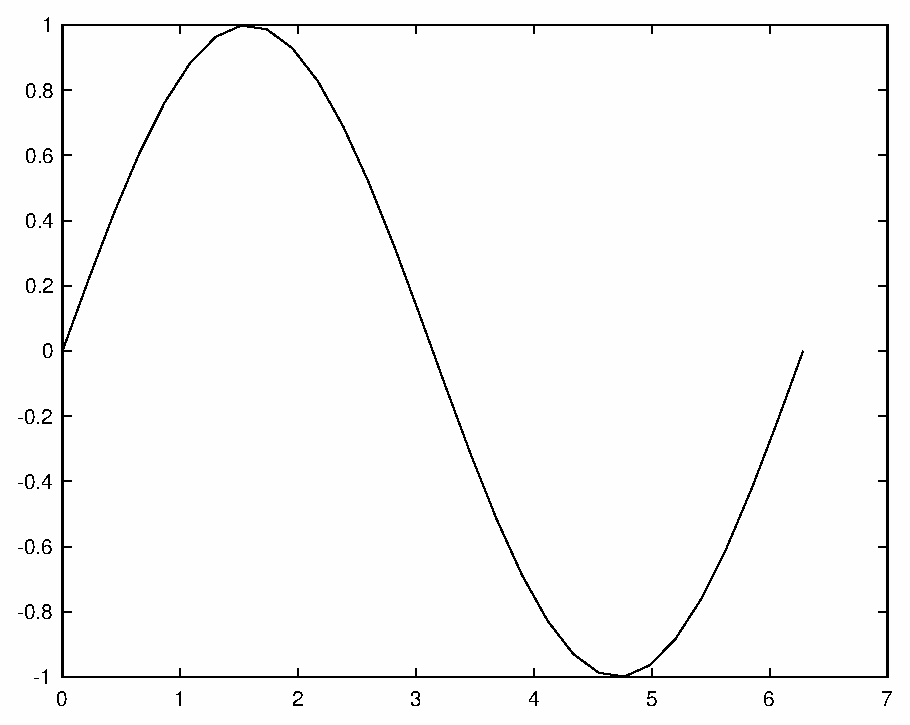
\includegraphics[scale=0.6]{hinhtieuluan/dothi1}
	\end{center}
		\caption{Đồ thị hàm số $y=\sin{x}$}
		\label{refdothi1}
	\end{figure}
\end{center}
Một cửa số mới sẽ được mở ra khi ta thực thi các dòng lệnh trên. Trong cửa sổ mới hiển thị đồ thị theo yêu cầu. Ta hoàn toàn có thể nhiều hàm số trong cùng một cửa sổ đồ thị như cách ta bổ sung thêm hàm $\cos{x}$ dưới đây:
\begin{lstlisting}
	>> z=cos(x);
	>> plot(x,y,x,z)
\end{lstlisting}
\begin{center}
	\begin{figure}[htp]
	\begin{center}
		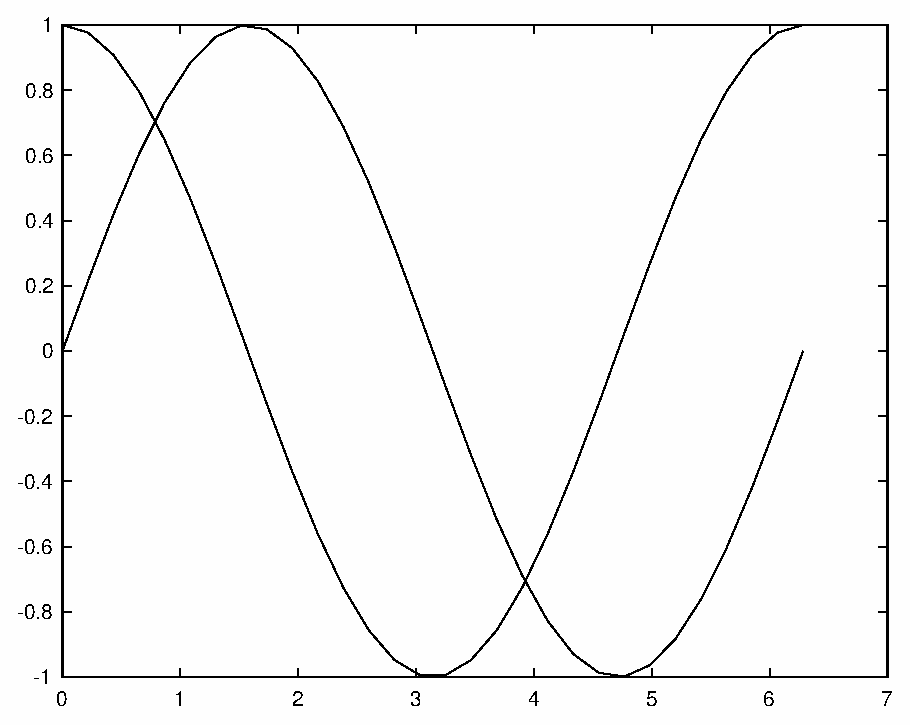
\includegraphics[scale=0.6]{hinhtieuluan/dothi2}
	\end{center}
		\caption{Đồ thị hàm số $y=\sin{x}$ và $z=\cos{x}$}
		\label{refdothi2}
	\end{figure}
\end{center}
Trong trường hợp một trong các đối số là ma trận và đối số còn lại là vectơ thì lệnh \chuyencode{plot} sẽ vẽ tương ứng mỗi cột của ma trận với vectơ đó. Cú pháp như bên dưới:
\begin{lstlisting}
	>> W=[y;z];
	>> plot(x,W)
\end{lstlisting}
\begin{center}
	\begin{figure}[htp]
	\begin{center}
		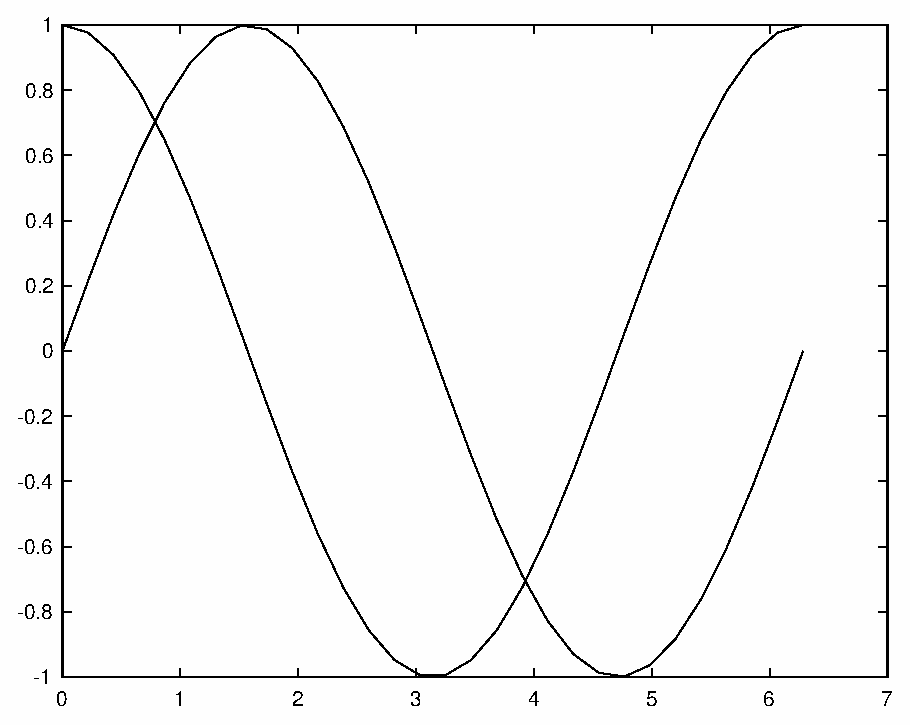
\includegraphics[scale=0.6]{hinhtieuluan/dothi3}
	\end{center}
		\caption{Đồ thị hàm số $y=\sin{x}$ và $z=\cos{x}$}
		\label{refdothi3}
	\end{figure}
\end{center}
Nếu người dùng thay đổi thứ tự các đối số thì đồ thị sẽ xoay một góc bằng 90 độ như bên dưới đây:
\begin{lstlisting}
	>> plot(W,x)
\end{lstlisting}
\begin{center}
	\begin{figure}[htp]
	\begin{center}
		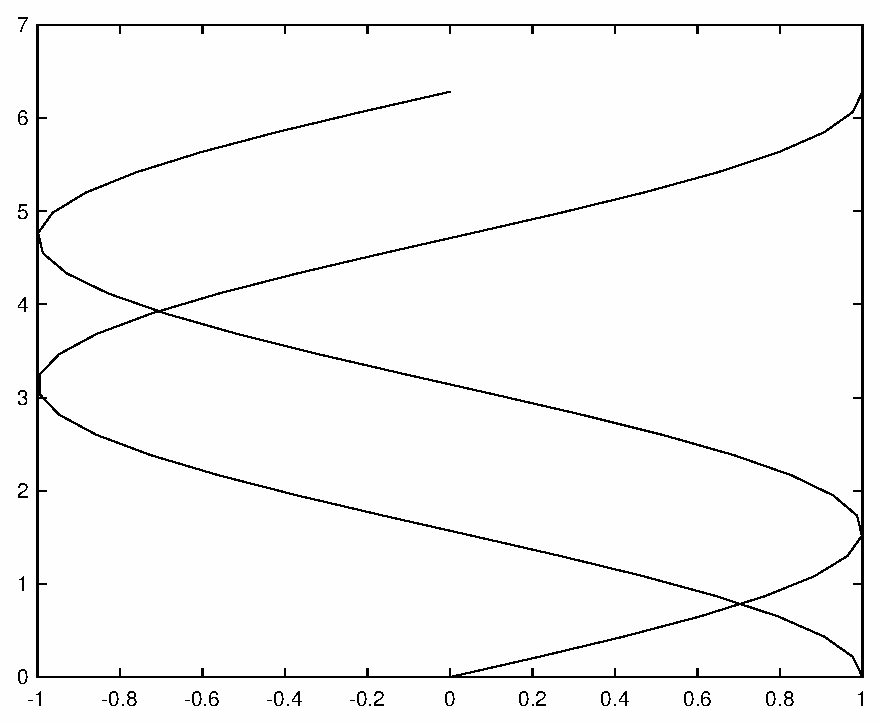
\includegraphics[scale=0.6]{hinhtieuluan/dothi4}
	\end{center}
		\caption{}
		\label{refdothi4}
	\end{figure}
\end{center}
\end{example}
\subsubsection{Kiểu đường, dấu và màu}
Mặc định MATLAB chọn màu đồ thị là \chuyencode{blue} và kiểu đường là \chuyencode{solid}. Người dùng có thể thay đổi kiểu dáng và màu sắc cho đồ thị thông qua các chuỗi đặc biệt được quy định như bản dưới đây:
\begin{table}[hp]
\centering
\label{bang3}
\begin{tabular}{|ll|ll|ll|}
\hline
\multicolumn{1}{|c|}{Biểu tượng} & \multicolumn{1}{c|}{Màu} & \multicolumn{1}{c|}{Biểu tượng} & \multicolumn{1}{c|}{Dấu} & \multicolumn{1}{c|}{Biểu tượng} & \multicolumn{1}{c|}{Kiểu nét vẽ} \\ \hline
\rowcolor[HTML]{DBDBDB} 
b                                & Xanh da trời             & .                               & Điểm                     & -                               & Nét liền                         \\
g                                & Xanh lá cây              & 0                               & Tròn                     & :                               & Đường chấm                       \\
\rowcolor[HTML]{DBDBDB} 
r                                & Đỏ                       & x                               & Dấu x                    & -.                              & Đường gạch chấm                  \\
c                                & Xanh xám                 & +                               & Dấu +                    & --                              & Đường gạch gạch                  \\
\rowcolor[HTML]{DBDBDB} 
m                                & Đỏ tím                   & *                               & Dấu *                    &                                 &                                  \\
y                                & Vàng                     & s                               & Vuông                    &                                 &                                  \\
\rowcolor[HTML]{DBDBDB} 
k                                & Đen                      & d                               & Diamond                  &                                 &                                  \\
w                                & Trắng                    & v                               & Triangle (down)          &                                 &                                  \\
\rowcolor[HTML]{DBDBDB} 
                                 &                          & \textasciicircum                & Triangle (up)            &                                 &                                  \\
                                 &                          & \textless                       & Triangle (left)          &                                 &                                  \\
\rowcolor[HTML]{DBDBDB} 
                                 &                          & \textgreater                    & Triangle (right)         &                                 &                                  \\
                                 &                          & p                               & Pentagram                &                                 &                                  \\
\rowcolor[HTML]{DBDBDB} 
                                 &                          & h                               & Hexagram                 &                                 &                                  \\ \hline
\end{tabular}
\end{table}\\
Ta thực hiện thay đổi kiểu đường và dấu vẽ đồ thị ở ví dụ trước đó như sau:
\begin{lstlisting}
	>> plot(x,y,'b:p',x,z,'c-',x,z,'m+')
\end{lstlisting}
\begin{center}
	\begin{figure}[H]
	\begin{center}
		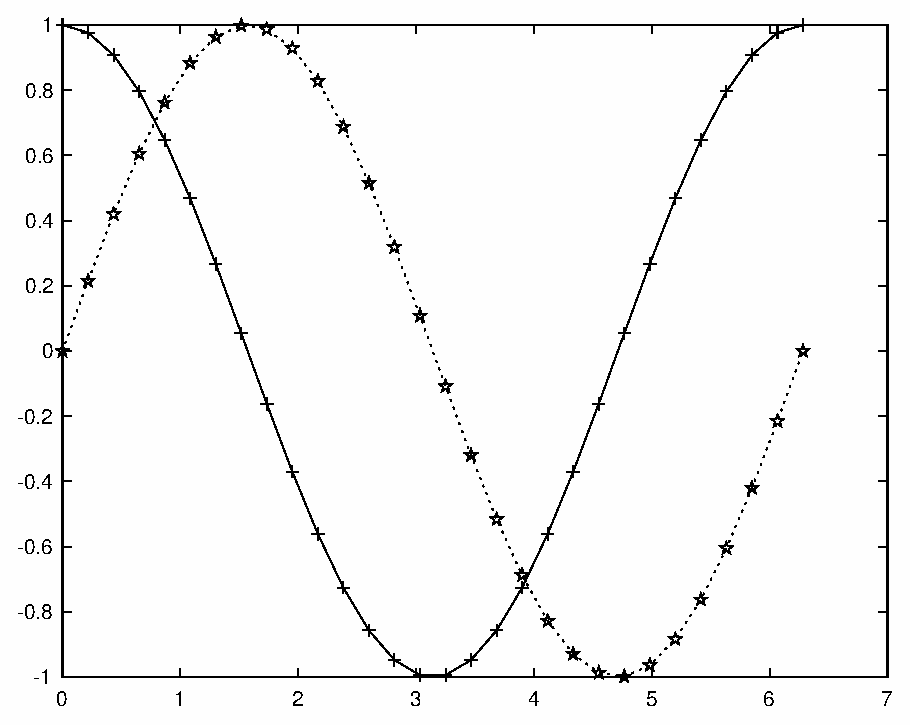
\includegraphics[scale=0.6]{hinhtieuluan/dothi5}
	\end{center}
		\caption{}
		\label{refdothi5}
	\end{figure}
\end{center}
\subsubsection{Kiểu đồ thị}
Lệnh \chuyencode{colordef} cho phép bạn lựa chọn kiểu hiển thị. Giá trị mặc định của \chuyencode{colordef} là \chuyencode{white}. Kiểu này sử dụng trục toạ độ, màu nền, nên hình vẽ màu xám sáng, và tên tiêu đề của trục màu đen. Người dùng có thể dùng lệnh \chuyencode{colordef black}, sẽ cho ra nền trục toạ độ đen, nền hình vẽ màu tối xám, và tiêu đề trục màu trắng
\subsubsection{Đồ thị lưới, hộp chức trục, nhãn và lời chú giải}
\begin{itemize}
	\item Lệnh \chuyencode{grid on} sẽ thêm đường lưới vào đồ thị hiện tại.
	\item Lệnh \chuyencode{grid off} sẽ bỏ các nét lưới đã thêm vào trước đó.
	\item Hộp viền ngoài toạ độ có thể tắt đi với \chuyencode{box off} và bật lại với \chuyencode{box on}.
	\item Gắn nhãn vào trục đứng với lệnh \chuyencode{ylabel}.
	\item Gắn nhãn vào trục ngang với lệnh \chuyencode{xlabel}.
	\item Thêm tiêu đề phía trên đồ thị với lệnh \chuyencode{title}.
\end{itemize}
Xét đồ thị $\sin{x}$ và $\cos{x}$ trước đó, ta thực hiện tạo lại đồ thị cơ bản như sau:
\begin{lstlisting}
	>> x=linspace(0,2*pi,30);
	>> y=sin(x);
	>> z=cos(x);
	>> plot(x,y,x,z)
\end{lstlisting}
\begin{center}
	\begin{figure}[H]
	\begin{center}
		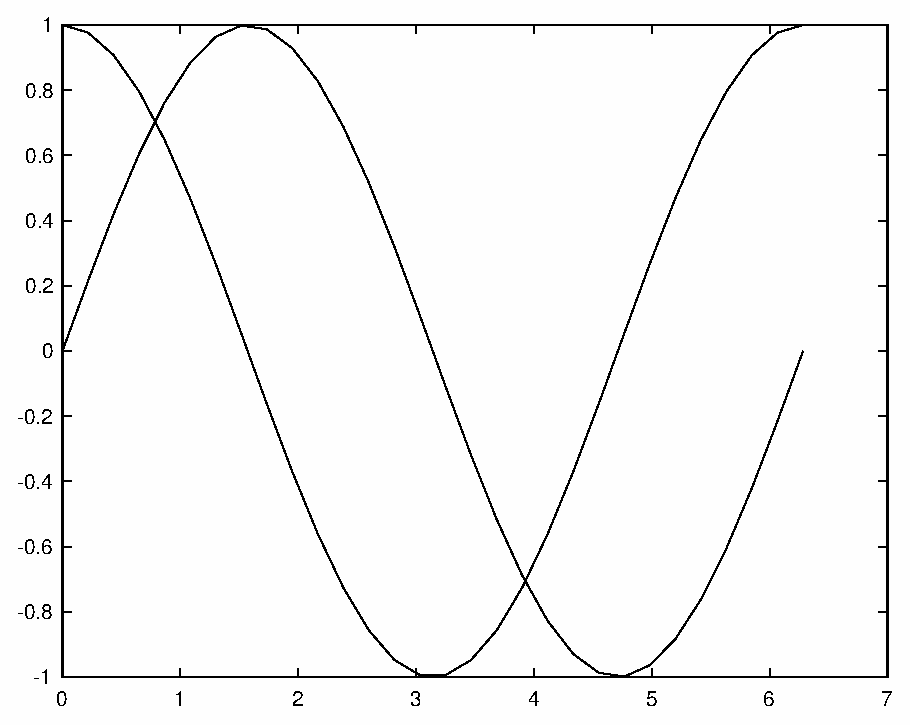
\includegraphics[scale=0.6]{hinhtieuluan/dothi2}
	\end{center}
		\caption{}
		\label{refdothi2}
	\end{figure}
\end{center}
Tiến hành tắt đi hộp viền ngoài trục toạ độ, đặt tên nhãn cho trục ngang, trục đứng và tiêu đề cho đồ thị như sau:
\begin{lstlisting}
	>> box off
	>> xlabel('Independent variable X')
	>> ylabel('Dependent variable Y and Z')
	>> title('Sine and Cosine Curve')
	>> print -deps dothi6
\end{lstlisting}
\begin{center}
	\begin{figure}[H]
	\begin{center}
		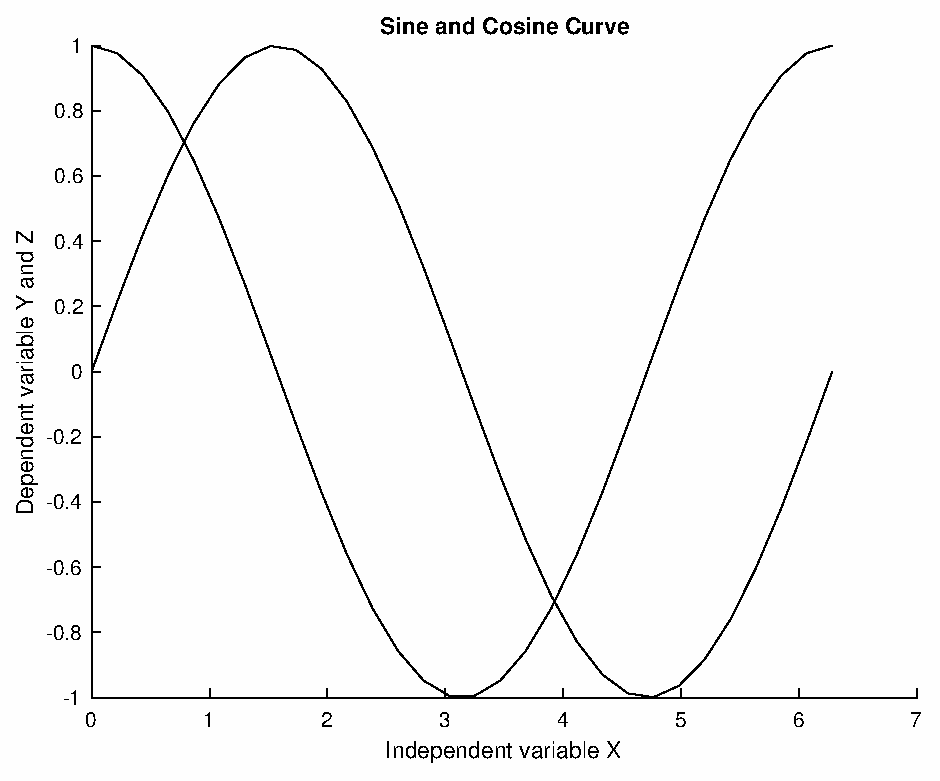
\includegraphics[scale=0.6]{hinhtieuluan/dothi6}
	\end{center}
		\caption{}
		\label{refdothi6}
	\end{figure}
\end{center}
Ngoài ra, người dùng có thể dùng lệnh \chuyencode{text(x,y,'string')} để thêm chú thích hay tên của đồ thị tại toạ độ x, y tuỳ ý. Nếu người dùng không muốn bỏ hình vẽ khỏi hệ trục đang xét, người dùng có thể thêm chuỗi văn bản bằng cách di chuột đến vị trị mong muốn. Lệnh \chuyencode{gtext} sẽ thực hiện việc này. Sau đây là ví dụ minh hoạ:
\begin{lstlisting}
	>> text(2.5,0.7,'sin(x)')
	>> gtext('cos(x)')
\end{lstlisting}
\begin{center}
	\begin{figure}[H]
	\begin{center}
		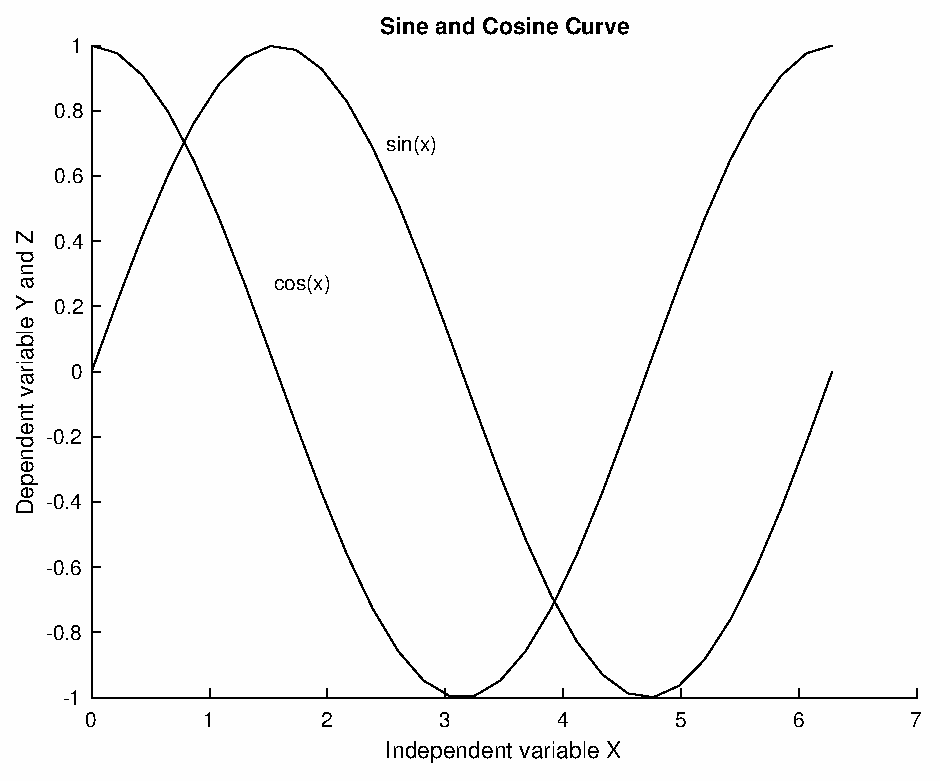
\includegraphics[scale=0.6]{hinhtieuluan/dothi7}
	\end{center}
		\caption{}
		\label{refdothi7}
	\end{figure}
\end{center}
\subsubsection{Kiến tạo hệ trục toạ độ}
Người dùng có thể chỉnh sửa thay đổi khoảng cách hay kiểu của trục đứng và trục ngang thông qua lệnh \chuyencode{axis}. Áp dụng vào đồ thị có sẵn từ ví dụ phần trước ta thực hành các lệnh cơ bản như:
\begin{itemize}
	\item Bỏ trục toạ độ.
\begin{lstlisting}
	>> axis off
\end{lstlisting}
\begin{center}
	\begin{figure}[H]
	\begin{center}
		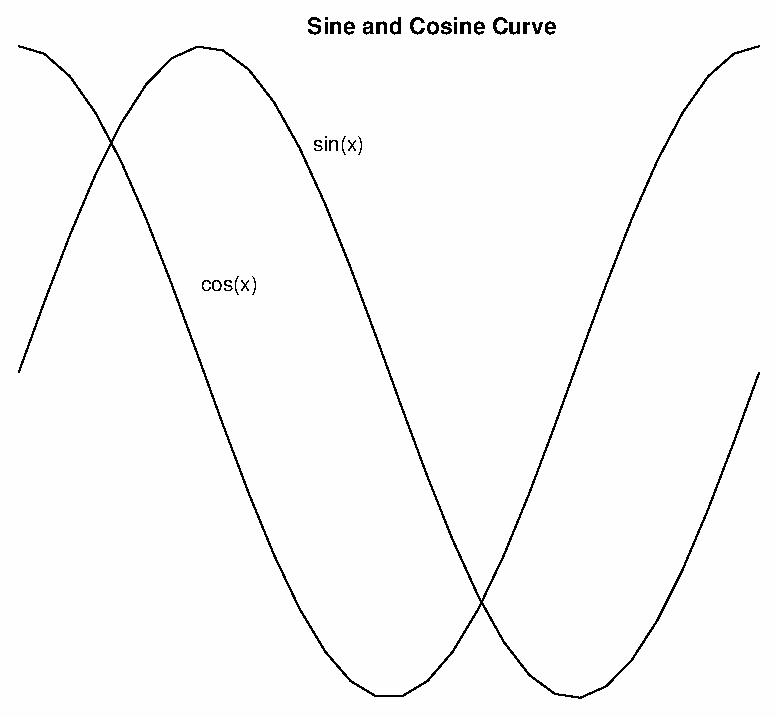
\includegraphics[scale=0.6]{hinhtieuluan/dothi8}
	\end{center}
		\caption{}
		\label{refdothi8}
	\end{figure}
\end{center}
	\item Bật trục toạ độ, tắt đường lưới.
\begin{lstlisting}
	>> axis on, grid off
\end{lstlisting}
\begin{center}
	\begin{figure}[H]
	\begin{center}
		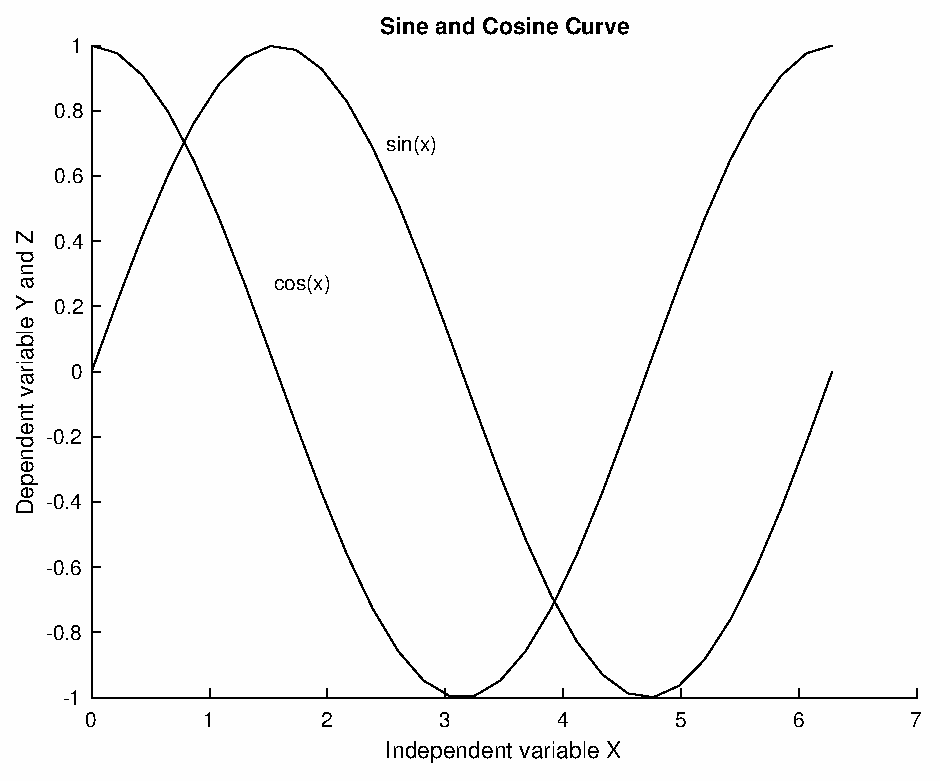
\includegraphics[scale=0.6]{hinhtieuluan/dothi9}
	\end{center}
		\caption{}
		\label{refdothi9}
	\end{figure}
\end{center}
	\item Lật ngược đồ thị.
\begin{lstlisting}
	>> axis ij
\end{lstlisting}
\begin{center}
	\begin{figure}[H]
	\begin{center}
		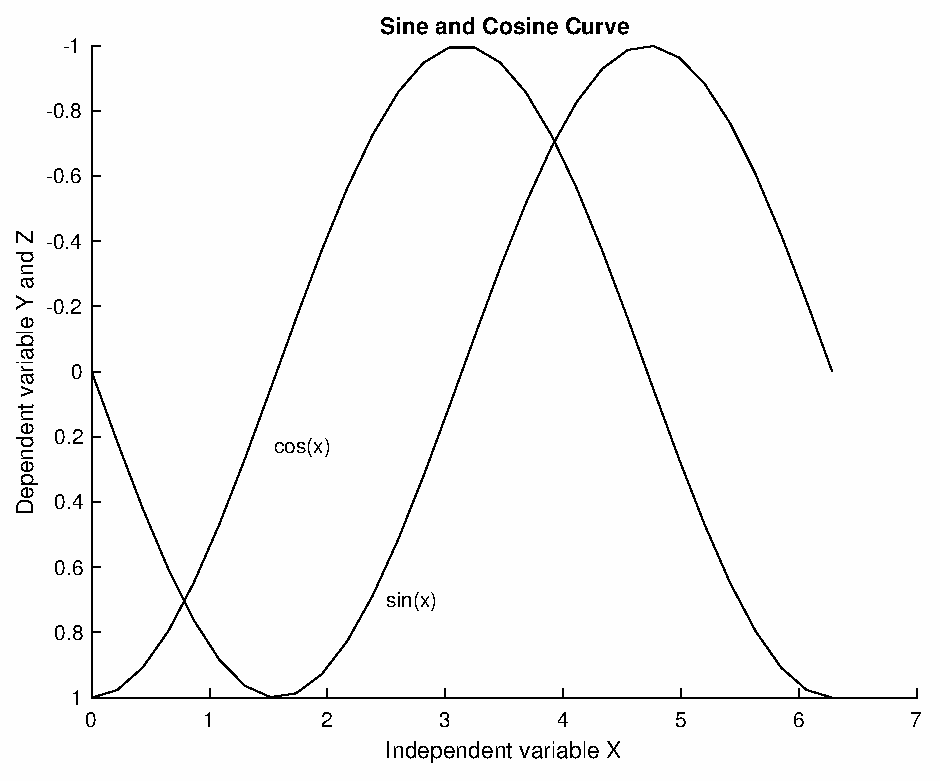
\includegraphics[scale=0.6]{hinhtieuluan/dothi10}
	\end{center}
		\caption{}
		\label{refdothi10}
	\end{figure}
\end{center}
	\item Thực hiện đồng thời thang chia trục như nhau và dạng đồ thị theo hình vuông.
\begin{lstlisting}
	>> axis square equal
\end{lstlisting}
\begin{center}
	\begin{figure}[H]
	\begin{center}
		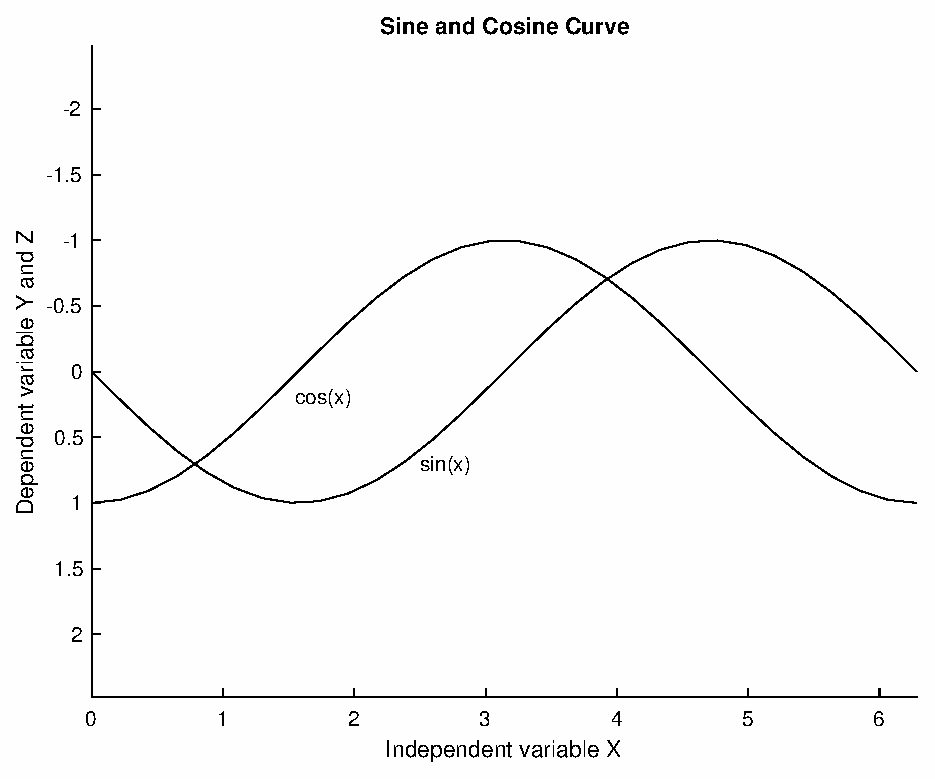
\includegraphics[scale=0.6]{hinhtieuluan/dothi11}
	\end{center}
		\caption{}
		\label{refdothi11}
	\end{figure}
\end{center}
	\item Trở về thiết lập mặc định.
\begin{lstlisting}
	>> axis xy normal
\end{lstlisting}
\begin{center}
	\begin{figure}[H]
	\begin{center}
		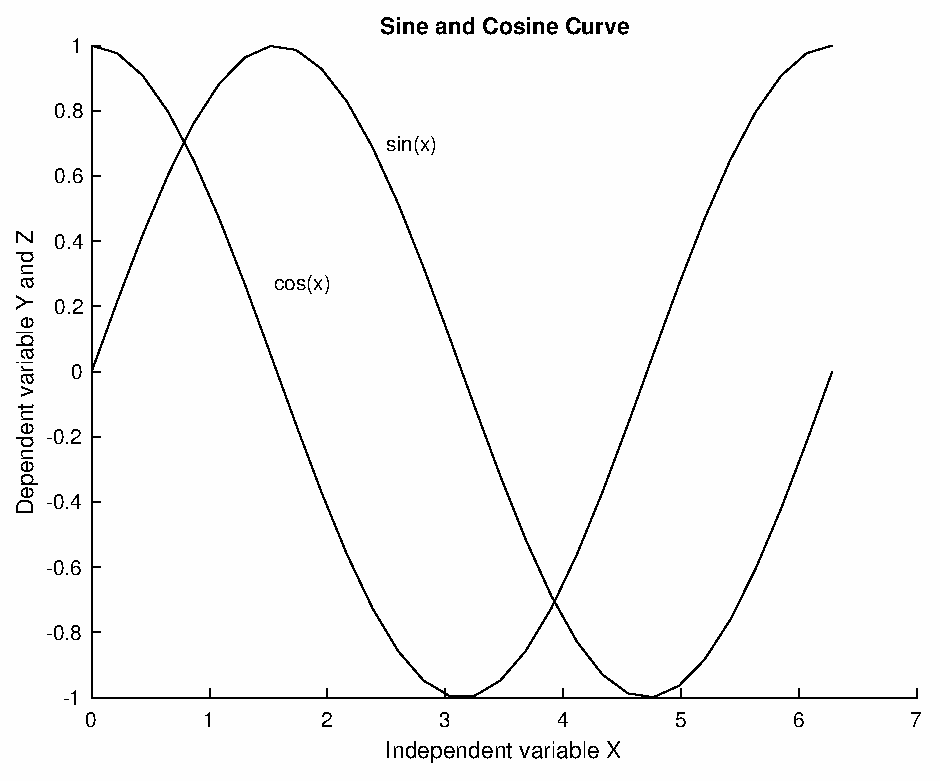
\includegraphics[scale=0.6]{hinhtieuluan/dothi12}
	\end{center}
		\caption{}
		\label{refdothi12}
	\end{figure}
\end{center}
\end{itemize}
\subsubsection{In hình}
Có hai cách để in hình hay đồ thị vừa vẽ là in từ cửa sổ hình vẽ  và in từ cửa sổ lệnh:
\begin{itemize}
	\item Thực hiện in hình từ cửa sổ chứa hình qua menu \menu{File>Print...}. Cửa sổ \textbf{Print} sẽ hiện ra và người dùng tiếp tục thao tác in ấn quen thuộc.
	\item Từ cửa sổ dòng lệnh, ta chọn hình cần in bằng lệnh \chuyencode{figure(n)}, với n là số thứ tự của hình cần in. sau đó ta dùng lệnh in với cú pháp:
\begin{lstlisting}
	>> print
\end{lstlisting}
	\item Ngoài hai cách trên, người dùng còn có thể in hình thành tệp ảnh có định dạng đuôi là eps để chèn vào nội dung tuỳ ý. Cú pháp như sau:
\begin{lstlisting}
	>> print -deps ten_hinh_anh
\end{lstlisting}
\end{itemize}
Ngoài ra người dùng còn có thể thay đổi kiểu in thông qua lệnh \chuyencode{orient} với các kiểu như sau:
\begin{itemize}
	\item Kiểu \chuyencode{portrait} in theo chiều đứng và hình nằm giữa trang.
	\item Kiểu \chuyencode{landspace} in theo chiều ngang và hình kín toàn bộ trang.
	\item Kiểu \chuyencode{tall} in theo chiều đứng nhưng hình kín toàn bộ trang.
\end{itemize}
Ta chỉ cần gõ cú pháp \chuyencode{orient kieu\_in} để thực hiện thay đổi kiểu in.
\subsubsection{Thao tác với đồ thị}
Ta có thể vẽ thêm hoặc tuỳ biến đồ thị mà không cần phải vẽ lại đồ thị nhiều lần bằng lệnh \chuyencode{hold}. Nhờ có lệnh \chuyencode{hold} mà người dùng có thể dùng lệnh \chuyencode{plot} liên tục mà không lo mất hình ảnh các đồ thị đã vẽ trước đó. Lệnh \chuyencode{ishold} trả về kết quả trạng thái của lệnh \chuyencode{hold} có hoạt động hay chưa. Xét ví dụ phần trước ta có:
\begin{lstlisting}
	>> x=linspace(0,2*pi,30);
	>> y=sin(x);
	>> z=cos(x);
	>> plot(x,y);
\end{lstlisting}
\begin{center}
	\begin{figure}[H]
	\begin{center}
		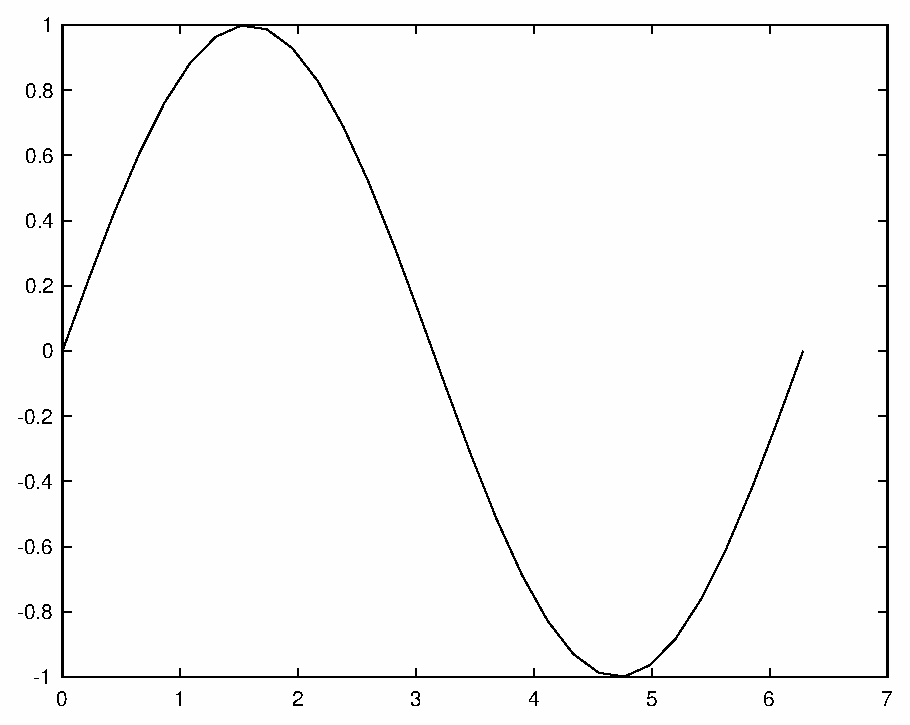
\includegraphics[scale=0.6]{hinhtieuluan/dothi1}
	\end{center}
		\caption{}
		\label{refdothi1}
	\end{figure}
\end{center}
Ta tiến hành giữ nguyên đồ thị bằng lệnh \chuyencode{hold} và vẽ thêm đồ thị $z=\cos{x}$ như sau:
\begin{lstlisting}
	>> hold on
	>> plot(x,z,'m*')
	>> hold off
\end{lstlisting}
\begin{center}
	\begin{figure}[H]
	\begin{center}
		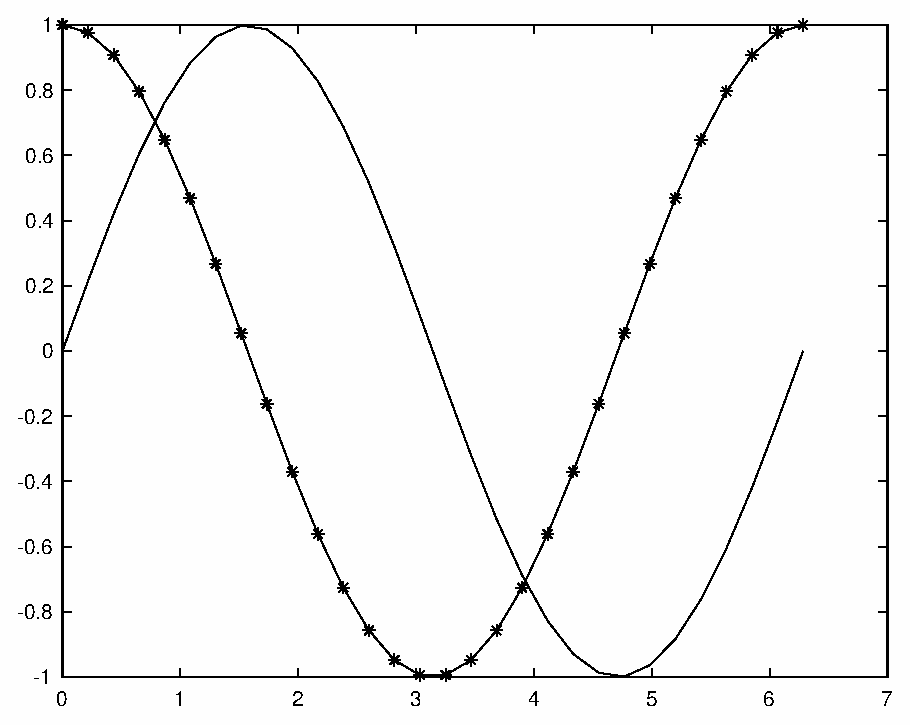
\includegraphics[scale=0.6]{hinhtieuluan/dothi13}
	\end{center}
		\caption{}
		\label{refdothi13}
	\end{figure}
\end{center}
\textbf{Lưu ý:} Một cửa sổ \textbf{figure} có thể chứa nhiều hệ trục toạ độ trong đó khi ta áp dụng lệnh \chuyencode{subplot(m,n,p)}. Trong đó, m và n chia cửa sổ thành một ma trận $mxn$ để vẽ đồ thị và p là cửa sổ hoạt động. Các đồ thị thành phần được đánh số thứ tự từ trái sang phải, từ trên xuống dưới.
\begin{example}
	Vẽ 4 đồ thị gồm $y=\sin{x} , z=\cos{x} , u=2 \sin{x} \cos{x} , v= \dfrac{\sin{x}}{\cos{x}}$ trong cùng một figure, trong đoạn $0 \leq x \leq 2\pi$ lấy 30 giá trị. Cú pháp như sau:
\begin{lstlisting}
	>> x=linspace(0,2*pi,30);
	>> y=sin(x);
	>> z=cos(x);
	>> u=2*sin(x).*cos(x);
	>> v=sin(x)./cos(x+eps);
	>> subplot(2,2,1)
	>> plot(x,y),axis([0,2*pi,-1,1]),title('sin(x)')
	>> subplot(2,2,2)
	>> plot(x,z),axis([0,2*pi,-1,1]),title('cos(x)')
	>> subplot(2,2,3)
	>> plot(x,u),axis([0,2*pi,-1,1]),title('2sin(x)cos(x)')
	>> subplot(2,2,4)
	>> plot(x,v),axis([0,2*pi,-20,20]),title('sin(x)/cos(x)')
\end{lstlisting}
\begin{center}
	\begin{figure}[H]
	\begin{center}
		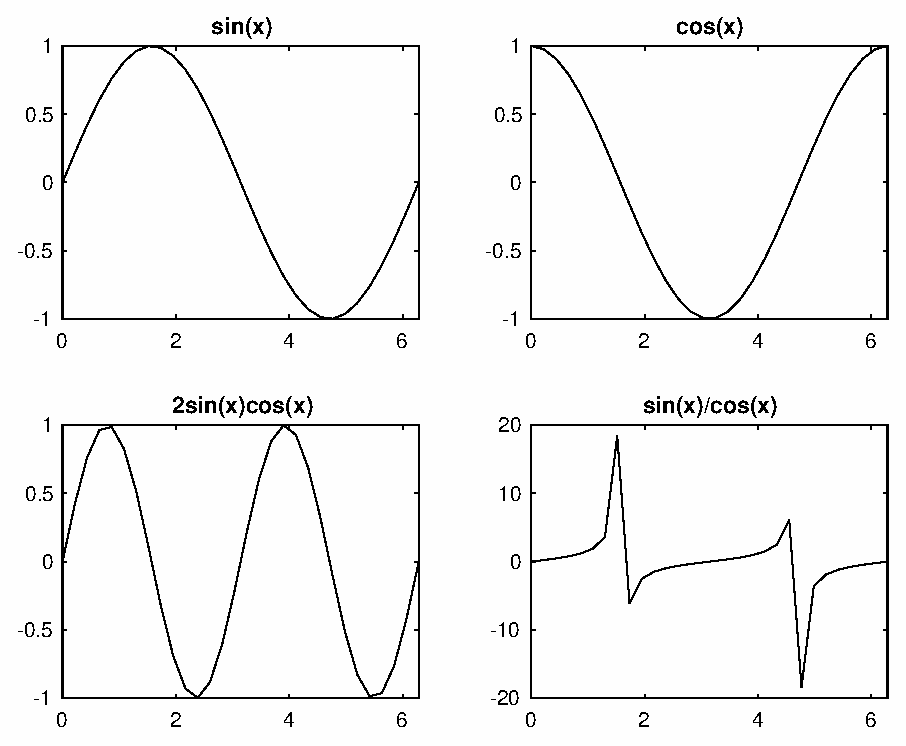
\includegraphics[scale=1]{hinhtieuluan/dothi14}
	\end{center}
		\caption{}
		\label{refdothi14}
	\end{figure}
\end{center}
\end{example}
\subsection{Đồ hoạ trong không gian ba chiều}
\subsubsection{Đồ thị đường thẳng}
Lệnh \chuyencode{plot} trong không gian hai chiều có thể mở rộng cho không gian 3 chiều bằng lệnh \chuyencode{plot3}. Cú pháp như sau:
\begin{lstlisting}
	>> plot3(x1,y1,z1,S1,x2,y2,z2,S2,...)
\end{lstlisting}
Trong đó các xn, yn và zn là các vectơ hoặc ma trận và Sn là xâu ký tự quy định dạng đồ thị (màu sắc, kiểu đường, kiểu đánh dấu...). Ví dụ một đồ thị trong không gian ba chiều như sau:
\begin{lstlisting}
	>> t=linspace(0,10*pi);
	>> plot3(sin(t),cos(t),t)
	>> title('Helix'),xlabel('sin(t)')
	>> ylabel('cos(t)'),zlabel('t')
\end{lstlisting}
\begin{center}
	\begin{figure}[H]
	\begin{center}
		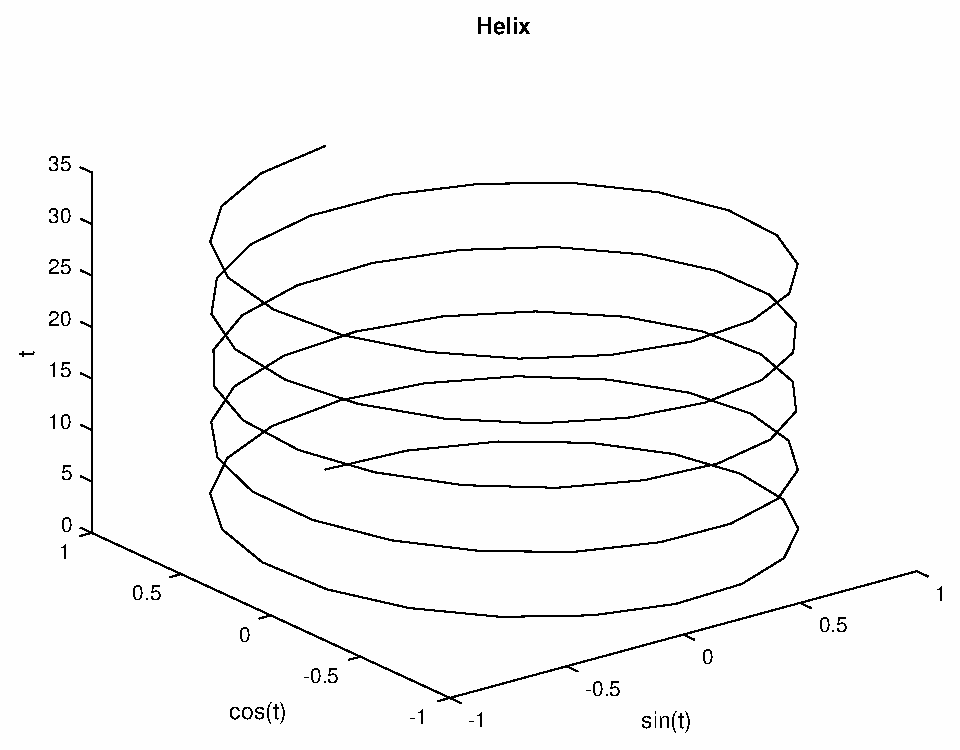
\includegraphics[scale=0.6]{hinhtieuluan/dothi15}
	\end{center}
		\caption{Đường Helix trong không gian ba chiều}
		\label{refdothi15}
	\end{figure}
\end{center}
Hàm \chuyencode{zlabel} tương ứng với hàm hai chiều là \chuyencode{xlabel} và \chuyencode{ylabel}. Thêm vào đó lệnh \chuyencode{axis} sẽ dùng cú pháp: \chuyencode{axis([xmin xmax ymin ymax zmin zmax])} để thiết lập giới hạn cho cả 3 trục.\\
Ngoài ra hàm \chuyencode{text} dùng cú pháp: \chuyencode{text(x,y,z,'string')} để đặt chuỗi văn bản vào toạ độ x, y, z theo ý muốn.
\subsubsection{Đồ thị bề mặt và lưới}
Hàm \chuyencode{meshgrid} tạo ma trận mới mà các hàng và cột là bản sao của hai ma trận cho trước. Cú pháp như sau: \chuyencode{[X,Y]=meshgrid(x,y)}. Sau đây là ví dụ cách dùng hàm \chuyencode{meshgrid}.
\begin{itemize}
	\item Tạo ma trận X, Y từ hàm \chuyencode{meshgrid}:
\begin{lstlisting}
	>> x=-7.5:.5:7.5;
	>> y=x;
	>> [X,Y]=meshgrid(x,y);
\end{lstlisting}	
	\item X, Y là một cặp ma trận tương ứng một lưới chữ nhật trong mặt phẳng x-y. Mọi hàm $z=f(x,y)$ có thể sử dụng tính chất này.
	\item Ma trận R chứa bán kính mỗi điểm trong [X,Y], nó là khoảng cách từ mỗi điểm đến tâm ma trận. Ta cộng thêm \textbf{eps} để không xảy ra phép chia cho 0. Ma trận Z chứa sin của bán kính chia cho bán kính mỗi điểm trong sơ đồ. Câu lệnh sau vẽ đồ thị  lưới:
\begin{lstlisting}
	>> R=sqrt(X.^2+Y.^2)+eps;
	>> Z=sin(R)./R;
	>> mesh(X,Y,Z)
\end{lstlisting}
\begin{center}
	\begin{figure}[H]
	\begin{center}
		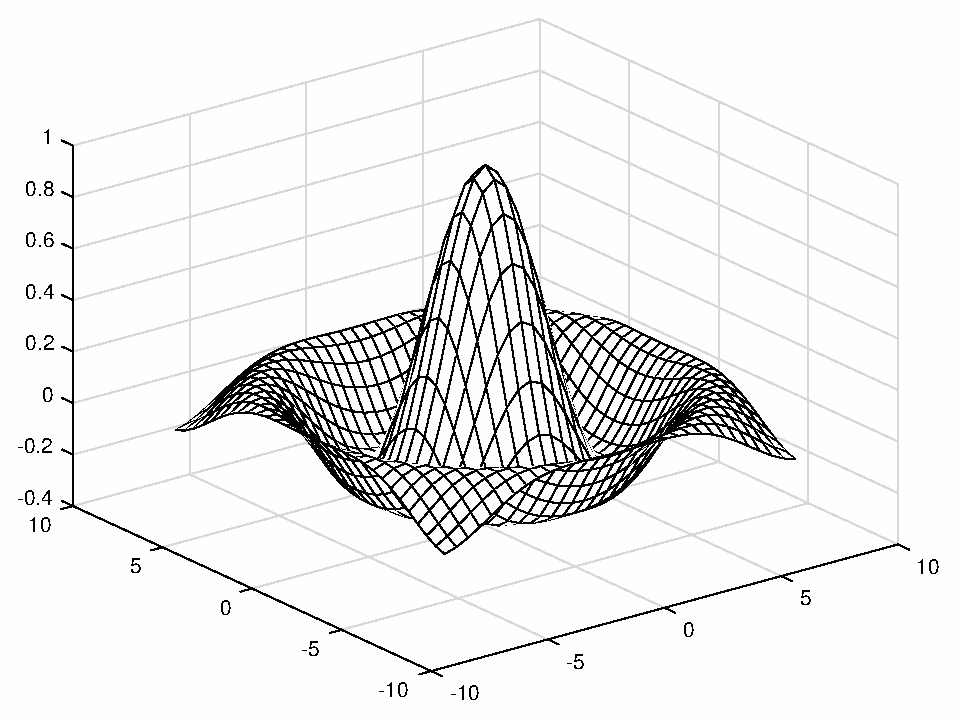
\includegraphics[scale=0.6]{hinhtieuluan/dothi16}
	\end{center}
		\caption{}
		\label{refdothi16}
	\end{figure}
\end{center}
\textbf{Lưu ý:} Đồ thị có thể tuỳ biến màu sắc trong phần \chuyencode{colormaps} của MATLAB.
\end{itemize}
Đồ thị bề mặt sử dụng lệnh \chuyencode{surf} để vẽ như sau:
\begin{lstlisting}
	>> surf(X,Y,Z)
\end{lstlisting}
\begin{center}
	\begin{figure}[H]
	\begin{center}
		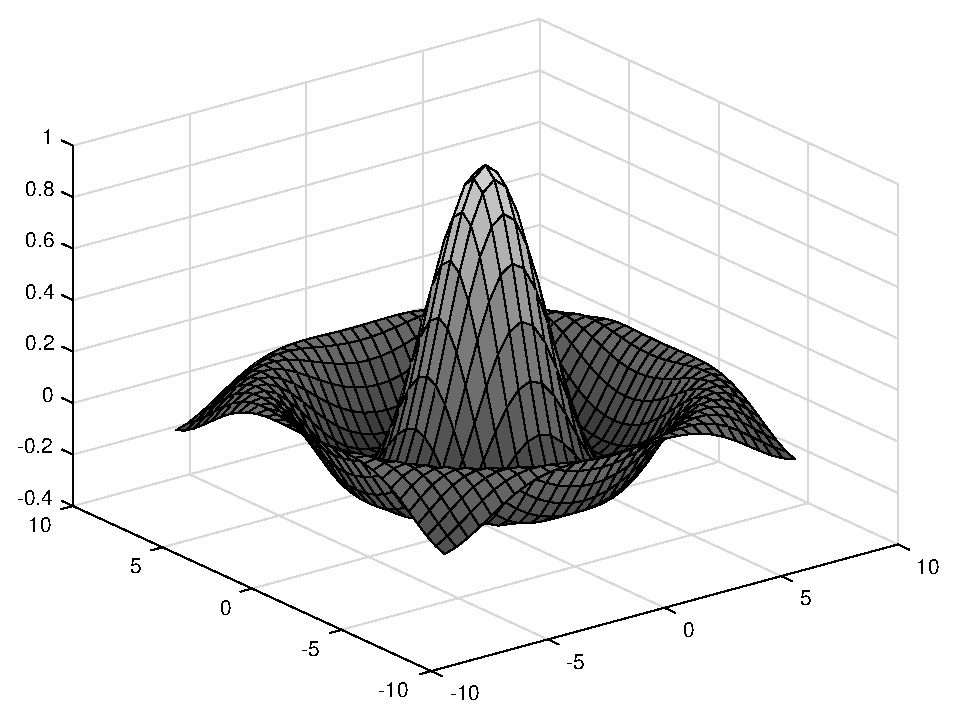
\includegraphics[scale=0.6]{hinhtieuluan/dothi17}
	\end{center}
		\caption{}
		\label{refdothi17}
	\end{figure}
\end{center}
Thêm một ví dụ nữa, ta dùng hàm \chuyencode{peaks} kết hợp với lệnh \chuyencode{mesh} như sau:
\begin{lstlisting}
	>> mesh(peaks)
	>> title('Mesh Plot of Peaks function')
\end{lstlisting}
\begin{center}
	\begin{figure}[H]
	\begin{center}
		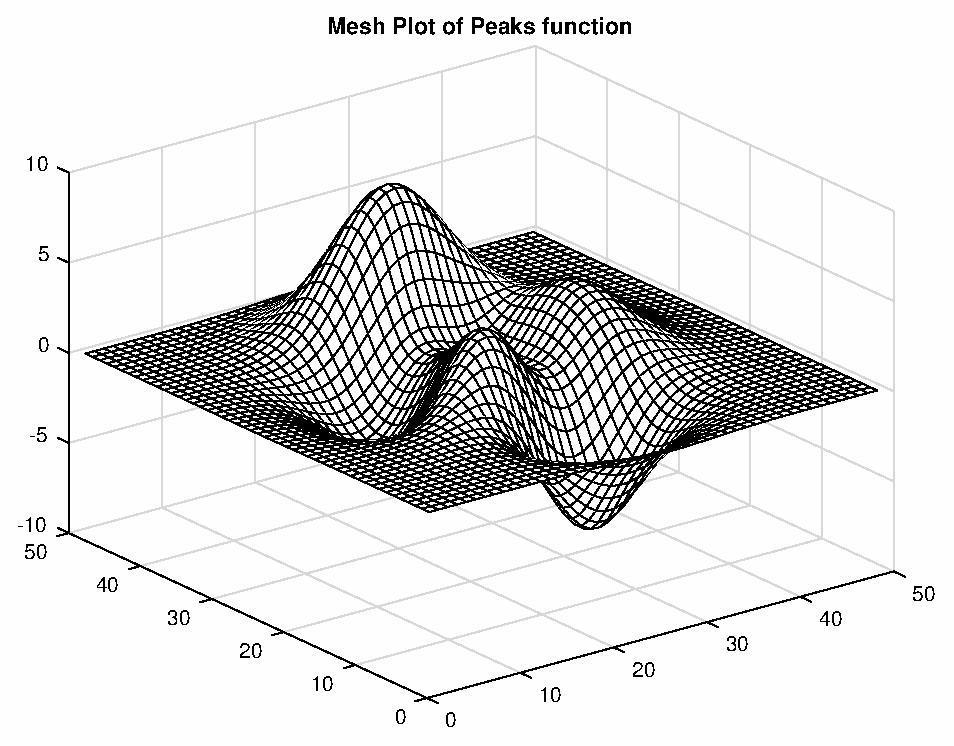
\includegraphics[scale=0.6]{hinhtieuluan/dothi18}
	\end{center}
		\caption{}
		\label{refdothi18}
	\end{figure}
\end{center}
\subsubsection{Thao tác với đồ thị}
MATLAB cho phép người dùng khai báo góc qua sát đồ thị trong không gian ba chiều. Hàm \chuyencode{view(azimuth, elevation)} thiết lập góc xem qua hai thành phần là \chuyencode{azimuth} (mô tả góc trong hệ trục nơi người qua sát đứng) và \chuyencode{elevation} (mô tả vị trí người quan sát).\\
Thành phần \chuyencode{azimuth} thiết lập dương thì hình sẽ quay ngược chiều kim đồng hồ từ điểm nhìn mặc định. Thành phần \chuyencode{elevation} nếu thiết lập là âm thì \chuyencode{view} sẽ nhìn hình từ phía dưới lên. Nếu muốn nhìn trực tiếp ta dùng lệnh \chuyencode{view(0,90)}. Ngoài ra, dạng \chuyencode{view(2)} cho ta góc xem hoàn toàn giống như mặc định của \chuyencode{view(0,90)} và dạng \chuyencode{view(3)} thiết lập mặc định trong không gian 3 chiều.
\begin{center}
	\begin{figure}[H]
	\begin{center}
		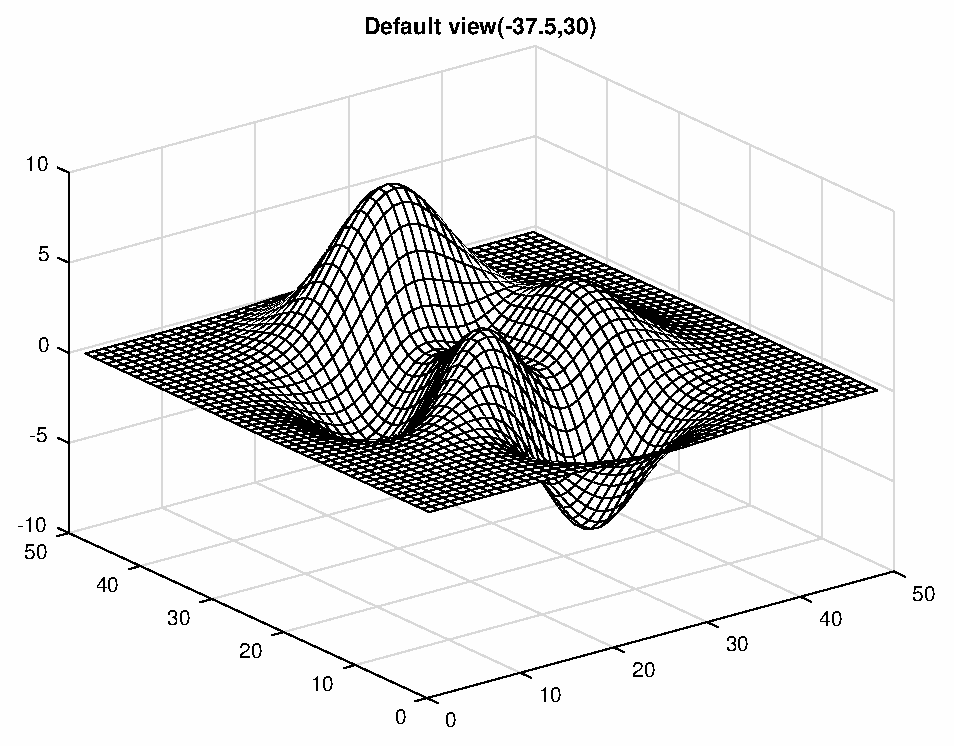
\includegraphics[scale=0.6]{hinhtieuluan/dothi19}
	\end{center}
		\caption{}
		\label{refdothi19}
	\end{figure}
\end{center}
\begin{center}
	\begin{figure}[H]
	\begin{center}
		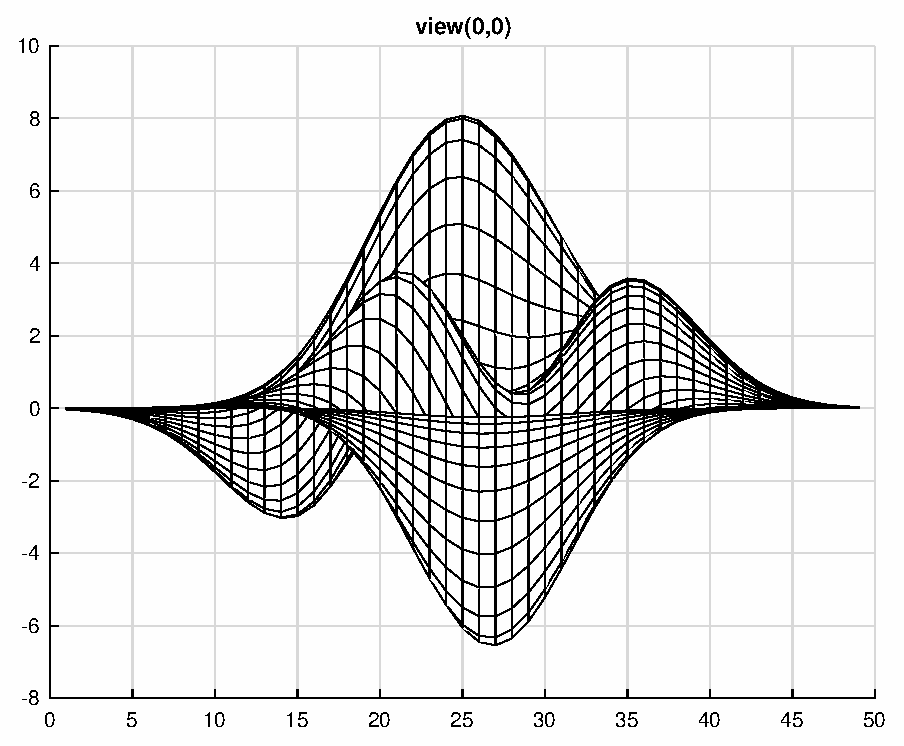
\includegraphics[scale=0.6]{hinhtieuluan/dothi20}
	\end{center}
		\caption{}
		\label{refdothi20}
	\end{figure}
\end{center}
Ngoài hai thành phần \chuyencode{azimuth} và \chuyencode{elevation}, người dùng còn có thể dùng trực tiếp toạ độ Đề-các bằng cú pháp: \chuyencode{view([X,Y,Z])}.\\
Hàm \chuyencode{rotate3d} cho phép dùng chuột can thiệp vào góc quan sát. Lệnh \chuyencode{hidden} sẽ ẩn đi các nét khuất. Cách dùng lệnh \chuyencode{hidden} như ví dụ dưới đây:
\begin{itemize}
	\item Thiết lập đồ thị ban đầu.
\begin{lstlisting}
	>> mesh(peaks(20)+7)
	>> hold on
	>> pcolor(peaks(20))
	>> hold off
	>> title('Mesh with hidden on')
\end{lstlisting}
\begin{center}
	\begin{figure}[H]
	\begin{center}
		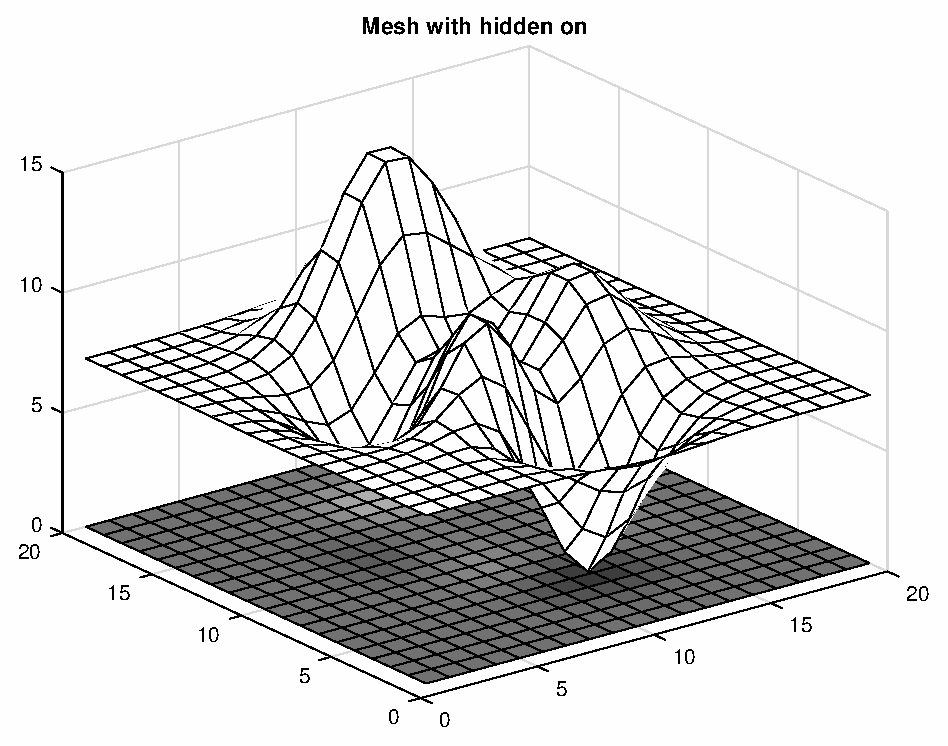
\includegraphics[scale=0.6]{hinhtieuluan/dothi21}
	\end{center}
		\caption{}
		\label{refdothi21}
	\end{figure}
\end{center}
	\item Chọn \chuyencode{hidden off}.
\begin{lstlisting}
	>> hidden off
	>> title('Mesh with Hidden Off')
\end{lstlisting}
\begin{center}
	\begin{figure}[H]
	\begin{center}
		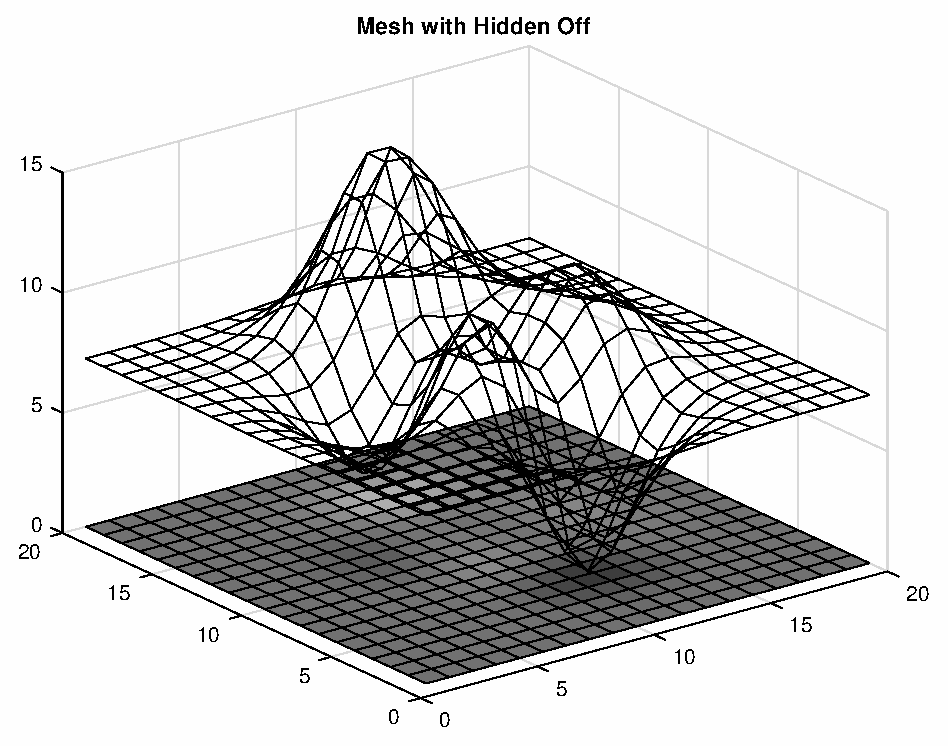
\includegraphics[scale=0.6]{hinhtieuluan/dothi22}
	\end{center}
		\caption{}
		\label{refdothi22}
	\end{figure}
\end{center}
\end{itemize}
\newpage
\listoffigures
\newpage
\begin{center}
	\textbf{TÀI LIỆU THAM KHẢO}\\

\end{center}
\end{document}